\documentclass[a4paper]{book}
\usepackage{makeidx}
\usepackage{natbib}
\usepackage{graphicx}
\usepackage{multicol}
\usepackage{float}
\usepackage{listings}
\usepackage{color}
\usepackage{ifthen}
\usepackage[table]{xcolor}
\usepackage{textcomp}
\usepackage{alltt}
\usepackage{ifpdf}
\ifpdf
\usepackage[pdftex,
            pagebackref=true,
            colorlinks=true,
            linkcolor=blue,
            unicode
           ]{hyperref}
\else
\usepackage[ps2pdf,
            pagebackref=true,
            colorlinks=true,
            linkcolor=blue,
            unicode
           ]{hyperref}
\usepackage{pspicture}
\fi
\usepackage[utf8]{inputenc}
\usepackage{mathptmx}
\usepackage[scaled=.90]{helvet}
\usepackage{courier}
\usepackage{sectsty}
\usepackage[titles]{tocloft}
\usepackage{doxygen}
\lstset{language=C++,inputencoding=utf8,basicstyle=\footnotesize,breaklines=true,breakatwhitespace=true,tabsize=8,numbers=left }
\makeindex
\setcounter{tocdepth}{3}
\renewcommand{\footrulewidth}{0.4pt}
\renewcommand{\familydefault}{\sfdefault}
\hfuzz=15pt
\setlength{\emergencystretch}{15pt}
\hbadness=750
\tolerance=750
\begin{document}
\hypersetup{pageanchor=false,citecolor=blue}
\begin{titlepage}
\vspace*{7cm}
\begin{center}
{\Large \-My \-Project }\\
\vspace*{1cm}
{\large \-Generated by Doxygen 1.7.6.1}\\
\vspace*{0.5cm}
{\small Thu Mar 19 2015 15:54:45}\\
\end{center}
\end{titlepage}
\clearemptydoublepage
\pagenumbering{roman}
\tableofcontents
\clearemptydoublepage
\pagenumbering{arabic}
\hypersetup{pageanchor=true,citecolor=blue}
\chapter{\-Namespace \-Index}
\section{\-Namespace \-List}
\-Here is a list of all documented namespaces with brief descriptions\-:\begin{DoxyCompactList}
\item\contentsline{section}{\hyperlink{namespaceCharacter}{\-Character} \\*\-File with \hyperlink{namespaceCharacter}{\-Character} class definition }{\pageref{namespaceCharacter}}{}
\item\contentsline{section}{\hyperlink{namespaceGameObject}{\-Game\-Object} \\*\-File containing \hyperlink{classGameObject_1_1Layer}{\-Layer} and \hyperlink{namespaceGameObject}{\-Game\-Object} class definitions }{\pageref{namespaceGameObject}}{}
\item\contentsline{section}{\hyperlink{namespaceInteraction}{\-Interaction} \\*\-File with \hyperlink{namespaceInteraction}{\-Interaction} class }{\pageref{namespaceInteraction}}{}
\item\contentsline{section}{\hyperlink{namespaceScript}{\-Script} \\*\-File with the \hyperlink{namespaceScript}{\-Script} class definition }{\pageref{namespaceScript}}{}
\item\contentsline{section}{\hyperlink{namespaceSpace}{\-Space} \\*\-File containing \hyperlink{classSpace_1_1Cell}{\-Cell}, \hyperlink{classSpace_1_1Grid}{\-Grid} and \hyperlink{classSpace_1_1GameSpace}{\-Game\-Space} class definitions }{\pageref{namespaceSpace}}{}
\item\contentsline{section}{\hyperlink{namespaceTeam}{\-Team} \\*\-File with the \hyperlink{namespaceTeam}{\-Team} class definition }{\pageref{namespaceTeam}}{}
\end{DoxyCompactList}

\chapter{\-Class \-Index}
\section{\-Class \-Hierarchy}
\-This inheritance list is sorted roughly, but not completely, alphabetically\-:\begin{DoxyCompactList}
\item \contentsline{section}{\-Space.\-Cell}{\pageref{classSpace_1_1Cell}}{}
\item \contentsline{section}{\-Collision.\-Collision}{\pageref{classCollision_1_1Collision}}{}
\item \contentsline{section}{\-Game.\-Game}{\pageref{classGame_1_1Game}}{}
\item \contentsline{section}{\-Game\-Object.\-Game\-Object}{\pageref{classGameObject_1_1GameObject}}{}
\begin{DoxyCompactList}
\item \contentsline{section}{\-Character.\-Character}{\pageref{classCharacter_1_1Character}}{}
\begin{DoxyCompactList}
\item \contentsline{section}{\-Player.\-Player}{\pageref{classPlayer_1_1Player}}{}
\end{DoxyCompactList}
\end{DoxyCompactList}
\item \contentsline{section}{\-Space.\-Game\-Space}{\pageref{classSpace_1_1GameSpace}}{}
\item \contentsline{section}{\-Space.\-Grid}{\pageref{classSpace_1_1Grid}}{}
\item \contentsline{section}{\-Interaction.\-Interaction}{\pageref{classInteraction_1_1Interaction}}{}
\item \contentsline{section}{\-Game\-Object.\-Layer}{\pageref{classGameObject_1_1Layer}}{}
\item \contentsline{section}{\-Game.\-Poll}{\pageref{classGame_1_1Poll}}{}
\item \contentsline{section}{\-Script.\-Script}{\pageref{classScript_1_1Script}}{}
\item \contentsline{section}{\-Team.\-Team}{\pageref{classTeam_1_1Team}}{}
\end{DoxyCompactList}

\chapter{\-Class \-Index}
\section{\-Class \-List}
\-Here are the classes, structs, unions and interfaces with brief descriptions\-:\begin{DoxyCompactList}
\item\contentsline{section}{\hyperlink{classSpace_1_1Cell}{\-Space.\-Cell} }{\pageref{classSpace_1_1Cell}}{}
\item\contentsline{section}{\hyperlink{classCharacter_1_1Character}{\-Character.\-Character} }{\pageref{classCharacter_1_1Character}}{}
\item\contentsline{section}{\hyperlink{classCollision_1_1Collision}{\-Collision.\-Collision} }{\pageref{classCollision_1_1Collision}}{}
\item\contentsline{section}{\hyperlink{classGame_1_1Game}{\-Game.\-Game} }{\pageref{classGame_1_1Game}}{}
\item\contentsline{section}{\hyperlink{classGameObject_1_1GameObject}{\-Game\-Object.\-Game\-Object} }{\pageref{classGameObject_1_1GameObject}}{}
\item\contentsline{section}{\hyperlink{classSpace_1_1GameSpace}{\-Space.\-Game\-Space} }{\pageref{classSpace_1_1GameSpace}}{}
\item\contentsline{section}{\hyperlink{classSpace_1_1Grid}{\-Space.\-Grid} }{\pageref{classSpace_1_1Grid}}{}
\item\contentsline{section}{\hyperlink{classInteraction_1_1Interaction}{\-Interaction.\-Interaction} }{\pageref{classInteraction_1_1Interaction}}{}
\item\contentsline{section}{\hyperlink{classGameObject_1_1Layer}{\-Game\-Object.\-Layer} }{\pageref{classGameObject_1_1Layer}}{}
\item\contentsline{section}{\hyperlink{classPlayer_1_1Player}{\-Player.\-Player} }{\pageref{classPlayer_1_1Player}}{}
\item\contentsline{section}{\hyperlink{classGame_1_1Poll}{\-Game.\-Poll} }{\pageref{classGame_1_1Poll}}{}
\item\contentsline{section}{\hyperlink{classScript_1_1Script}{\-Script.\-Script} }{\pageref{classScript_1_1Script}}{}
\item\contentsline{section}{\hyperlink{classTeam_1_1Team}{\-Team.\-Team} }{\pageref{classTeam_1_1Team}}{}
\end{DoxyCompactList}

\chapter{\-Namespace \-Documentation}
\hypertarget{namespaceCharacter}{\section{\-Character \-Namespace \-Reference}
\label{namespaceCharacter}\index{\-Character@{\-Character}}
}


\-File with \hyperlink{namespaceCharacter}{\-Character} class definition.  


\subsection*{\-Classes}
\begin{DoxyCompactItemize}
\item 
class \hyperlink{classCharacter_1_1Character}{\-Character}
\end{DoxyCompactItemize}


\subsection{\-Detailed \-Description}
\-File with \hyperlink{namespaceCharacter}{\-Character} class definition. 
\hypertarget{namespaceGameObject}{\section{\-Game\-Object \-Namespace \-Reference}
\label{namespaceGameObject}\index{\-Game\-Object@{\-Game\-Object}}
}


\-File containing \hyperlink{classGameObject_1_1Layer}{\-Layer} and \hyperlink{namespaceGameObject}{\-Game\-Object} class definitions.  


\subsection*{\-Classes}
\begin{DoxyCompactItemize}
\item 
class \hyperlink{classGameObject_1_1Layer}{\-Layer}
\item 
class \hyperlink{classGameObject_1_1GameObject}{\-Game\-Object}
\end{DoxyCompactItemize}
\subsection*{\-Variables}
\begin{DoxyCompactItemize}
\item 
\hypertarget{namespaceGameObject_a882b48dfb1cfe58bddbcab47f72509f0}{string {\bfseries layerassert} = \char`\"{}\-Layer.\char`\"{}}\label{namespaceGameObject_a882b48dfb1cfe58bddbcab47f72509f0}

\item 
\hypertarget{namespaceGameObject_aa7de38f4a13f622a77d0471dc95823a2}{string {\bfseries gameobjectassert} = \char`\"{}\-Game\-Object.\char`\"{}}\label{namespaceGameObject_aa7de38f4a13f622a77d0471dc95823a2}

\end{DoxyCompactItemize}


\subsection{\-Detailed \-Description}
\-File containing \hyperlink{classGameObject_1_1Layer}{\-Layer} and \hyperlink{namespaceGameObject}{\-Game\-Object} class definitions. 
\hypertarget{namespaceInteraction}{\section{\-Interaction \-Namespace \-Reference}
\label{namespaceInteraction}\index{\-Interaction@{\-Interaction}}
}


\-File with \hyperlink{namespaceInteraction}{\-Interaction} class.  


\subsection*{\-Classes}
\begin{DoxyCompactItemize}
\item 
class \hyperlink{classInteraction_1_1Interaction}{\-Interaction}
\end{DoxyCompactItemize}
\subsection*{\-Variables}
\begin{DoxyCompactItemize}
\item 
\hypertarget{namespaceInteraction_a04a1df5923e2b51611886c109178fb52}{string {\bfseries interactionassert} = \char`\"{}\-Interaction.\char`\"{}}\label{namespaceInteraction_a04a1df5923e2b51611886c109178fb52}

\end{DoxyCompactItemize}


\subsection{\-Detailed \-Description}
\-File with \hyperlink{namespaceInteraction}{\-Interaction} class. 
\hypertarget{namespaceScript}{\section{\-Script \-Namespace \-Reference}
\label{namespaceScript}\index{\-Script@{\-Script}}
}


\-File with the \hyperlink{namespaceScript}{\-Script} class definition.  


\subsection*{\-Classes}
\begin{DoxyCompactItemize}
\item 
class \hyperlink{classScript_1_1Script}{\-Script}
\end{DoxyCompactItemize}
\subsection*{\-Variables}
\begin{DoxyCompactItemize}
\item 
\hypertarget{namespaceScript_a39acc8ebded1c4c225acea4ab18398b1}{string {\bfseries scriptassert} = \char`\"{}\-Script.\char`\"{}}\label{namespaceScript_a39acc8ebded1c4c225acea4ab18398b1}

\end{DoxyCompactItemize}


\subsection{\-Detailed \-Description}
\-File with the \hyperlink{namespaceScript}{\-Script} class definition. 
\hypertarget{namespaceSpace}{\section{\-Space \-Namespace \-Reference}
\label{namespaceSpace}\index{\-Space@{\-Space}}
}


\-File containing \hyperlink{classSpace_1_1Cell}{\-Cell}, \hyperlink{classSpace_1_1Grid}{\-Grid} and \hyperlink{classSpace_1_1GameSpace}{\-Game\-Space} class definitions.  


\subsection*{\-Classes}
\begin{DoxyCompactItemize}
\item 
class \hyperlink{classSpace_1_1Cell}{\-Cell}
\item 
class \hyperlink{classSpace_1_1Grid}{\-Grid}
\item 
class \hyperlink{classSpace_1_1GameSpace}{\-Game\-Space}
\end{DoxyCompactItemize}
\subsection*{\-Variables}
\begin{DoxyCompactItemize}
\item 
\hypertarget{namespaceSpace_a5b22449e08fb442d7bdc083428789714}{int {\bfseries \-X} = 0}\label{namespaceSpace_a5b22449e08fb442d7bdc083428789714}

\item 
\hypertarget{namespaceSpace_a1af791a727f2219ecd44e12aa8868872}{int {\bfseries \-Y} = 1}\label{namespaceSpace_a1af791a727f2219ecd44e12aa8868872}

\item 
\hypertarget{namespaceSpace_a61fa8c21f1a46663cd92d9256532154e}{int {\bfseries \-Z} = 2}\label{namespaceSpace_a61fa8c21f1a46663cd92d9256532154e}

\item 
\hypertarget{namespaceSpace_adb882bf3b26a5b4f7210bc9dead16334}{int {\bfseries \-D3} = 3}\label{namespaceSpace_adb882bf3b26a5b4f7210bc9dead16334}

\item 
\hypertarget{namespaceSpace_a9c552ca3d1e992e9cf4bf6656bfe1fc3}{int {\bfseries \-D2} = 2}\label{namespaceSpace_a9c552ca3d1e992e9cf4bf6656bfe1fc3}

\item 
\hypertarget{namespaceSpace_a24dce6fc17c893a134d136b8361ee25a}{string {\bfseries cellassert} = \char`\"{}\-Cell.\char`\"{}}\label{namespaceSpace_a24dce6fc17c893a134d136b8361ee25a}

\item 
\hypertarget{namespaceSpace_a1b2e0dd9dbd4679c9731efad20da31d3}{string {\bfseries gridassert} = \char`\"{}\-Grid.\char`\"{}}\label{namespaceSpace_a1b2e0dd9dbd4679c9731efad20da31d3}

\item 
\hypertarget{namespaceSpace_a927a89dd4c2b7d7c2aef66dbdb2b1fce}{string {\bfseries gamespaceassert} = \char`\"{}\-Game\-Space.\char`\"{}}\label{namespaceSpace_a927a89dd4c2b7d7c2aef66dbdb2b1fce}

\end{DoxyCompactItemize}


\subsection{\-Detailed \-Description}
\-File containing \hyperlink{classSpace_1_1Cell}{\-Cell}, \hyperlink{classSpace_1_1Grid}{\-Grid} and \hyperlink{classSpace_1_1GameSpace}{\-Game\-Space} class definitions. 
\hypertarget{namespaceTeam}{\section{\-Team \-Namespace \-Reference}
\label{namespaceTeam}\index{\-Team@{\-Team}}
}


\-File with the \hyperlink{namespaceTeam}{\-Team} class definition.  


\subsection*{\-Classes}
\begin{DoxyCompactItemize}
\item 
class \hyperlink{classTeam_1_1Team}{\-Team}
\end{DoxyCompactItemize}
\subsection*{\-Variables}
\begin{DoxyCompactItemize}
\item 
\hypertarget{namespaceTeam_a1678d14befad72a7125974f7a549ec2f}{string {\bfseries teamassert} = \char`\"{}\-Team.\char`\"{}}\label{namespaceTeam_a1678d14befad72a7125974f7a549ec2f}

\end{DoxyCompactItemize}


\subsection{\-Detailed \-Description}
\-File with the \hyperlink{namespaceTeam}{\-Team} class definition. 
\chapter{\-Class \-Documentation}
\hypertarget{classSpace_1_1Cell}{\section{\-Space.\-Cell \-Class \-Reference}
\label{classSpace_1_1Cell}\index{\-Space.\-Cell@{\-Space.\-Cell}}
}
\subsection*{\-Public \-Member \-Functions}
\begin{DoxyCompactItemize}
\item 
def \hyperlink{classSpace_1_1Cell_a924291fc11b25771ca67349d046eced5}{\-\_\-\-\_\-init\-\_\-\-\_\-}
\item 
def \hyperlink{classSpace_1_1Cell_a4ca073a5587452ac2efc91a5281e7e55}{center}
\item 
def \hyperlink{classSpace_1_1Cell_a0e044b5a744e0e7756fb9be0f7a0d1ff}{add\-Object}
\item 
def \hyperlink{classSpace_1_1Cell_ae42d3c27c10761a26288b2a3e4127873}{remove\-Object}
\item 
def \hyperlink{classSpace_1_1Cell_a4ce4dbf71e809f6f0e73a45adf3d8fac}{get\-Objects}
\item 
def \hyperlink{classSpace_1_1Cell_a2f4efef93b8307f4c0856ebd99171155}{introduction}
\item 
def \hyperlink{classSpace_1_1Cell_aaf19831256434c36cc7408936db65bfe}{catching\-Up}
\end{DoxyCompactItemize}
\subsection*{\-Public \-Attributes}
\begin{DoxyCompactItemize}
\item 
\hypertarget{classSpace_1_1Cell_a69795f2c1ed435d84d64b209be46a30e}{\hyperlink{classSpace_1_1Cell_a69795f2c1ed435d84d64b209be46a30e}{xb}}\label{classSpace_1_1Cell_a69795f2c1ed435d84d64b209be46a30e}

\begin{DoxyCompactList}\small\item\em x begin, lowest x coordinate that is in the cell \end{DoxyCompactList}\item 
\hypertarget{classSpace_1_1Cell_a1bfa638e3faed349d2d88438d8c57452}{\hyperlink{classSpace_1_1Cell_a1bfa638e3faed349d2d88438d8c57452}{xe}}\label{classSpace_1_1Cell_a1bfa638e3faed349d2d88438d8c57452}

\begin{DoxyCompactList}\small\item\em x end, highest x coordinate that is in the cell \end{DoxyCompactList}\item 
\hypertarget{classSpace_1_1Cell_aacd06f2c6f6e331d4ec03f93e62fa6d6}{\hyperlink{classSpace_1_1Cell_aacd06f2c6f6e331d4ec03f93e62fa6d6}{yb}}\label{classSpace_1_1Cell_aacd06f2c6f6e331d4ec03f93e62fa6d6}

\begin{DoxyCompactList}\small\item\em y begin, lowest y coordinate that is in the cell \end{DoxyCompactList}\item 
\hypertarget{classSpace_1_1Cell_a67848a0ad69098bdb539b063de16bab9}{\hyperlink{classSpace_1_1Cell_a67848a0ad69098bdb539b063de16bab9}{ye}}\label{classSpace_1_1Cell_a67848a0ad69098bdb539b063de16bab9}

\begin{DoxyCompactList}\small\item\em y end, highest y coordinate that is in the cell \end{DoxyCompactList}\item 
\hypertarget{classSpace_1_1Cell_a38b3f9f8f3c04995fb5f3c48e15229ba}{\hyperlink{classSpace_1_1Cell_a38b3f9f8f3c04995fb5f3c48e15229ba}{gameobjects}}\label{classSpace_1_1Cell_a38b3f9f8f3c04995fb5f3c48e15229ba}

\begin{DoxyCompactList}\small\item\em \-List of \-Game\-Objects (\hyperlink{namespaceGameObject}{\-Game\-Object}) currently in the \hyperlink{classSpace_1_1Cell}{\-Cell}. \end{DoxyCompactList}\end{DoxyCompactItemize}


\subsection{\-Detailed \-Description}
\begin{DoxyVerb}a Grid object's cell\end{DoxyVerb}
 

\subsection{\-Constructor \& \-Destructor \-Documentation}
\hypertarget{classSpace_1_1Cell_a924291fc11b25771ca67349d046eced5}{\index{\-Space\-::\-Cell@{\-Space\-::\-Cell}!\-\_\-\-\_\-init\-\_\-\-\_\-@{\-\_\-\-\_\-init\-\_\-\-\_\-}}
\index{\-\_\-\-\_\-init\-\_\-\-\_\-@{\-\_\-\-\_\-init\-\_\-\-\_\-}!Space::Cell@{\-Space\-::\-Cell}}
\subsubsection[{\-\_\-\-\_\-init\-\_\-\-\_\-}]{\setlength{\rightskip}{0pt plus 5cm}def {\bf \-Space.\-Cell.\-\_\-\-\_\-init\-\_\-\-\_\-} (
\begin{DoxyParamCaption}
\item[{}]{self, }
\item[{}]{xb, }
\item[{}]{xe, }
\item[{}]{yb, }
\item[{}]{ye}
\end{DoxyParamCaption}
)}}\label{classSpace_1_1Cell_a924291fc11b25771ca67349d046eced5}
\begin{DoxyVerb}Cell.__init__(self, xb, xe, yb, ye)
Initialization function for a Cell Object

xb is xbegin
xe in xend

same for yb and ye
\end{DoxyVerb}
 

\subsection{\-Member \-Function \-Documentation}
\hypertarget{classSpace_1_1Cell_a0e044b5a744e0e7756fb9be0f7a0d1ff}{\index{\-Space\-::\-Cell@{\-Space\-::\-Cell}!add\-Object@{add\-Object}}
\index{add\-Object@{add\-Object}!Space::Cell@{\-Space\-::\-Cell}}
\subsubsection[{add\-Object}]{\setlength{\rightskip}{0pt plus 5cm}def {\bf \-Space.\-Cell.\-add\-Object} (
\begin{DoxyParamCaption}
\item[{}]{self, }
\item[{}]{obj}
\end{DoxyParamCaption}
)}}\label{classSpace_1_1Cell_a0e044b5a744e0e7756fb9be0f7a0d1ff}
\begin{DoxyVerb}Cell.addObject(obj)
adds a GameObject obj to the cell's gameobjects[].
Returns True for success and False for failure
\end{DoxyVerb}
 \hypertarget{classSpace_1_1Cell_aaf19831256434c36cc7408936db65bfe}{\index{\-Space\-::\-Cell@{\-Space\-::\-Cell}!catching\-Up@{catching\-Up}}
\index{catching\-Up@{catching\-Up}!Space::Cell@{\-Space\-::\-Cell}}
\subsubsection[{catching\-Up}]{\setlength{\rightskip}{0pt plus 5cm}def {\bf \-Space.\-Cell.\-catching\-Up} (
\begin{DoxyParamCaption}
\item[{}]{self}
\end{DoxyParamCaption}
)}}\label{classSpace_1_1Cell_aaf19831256434c36cc7408936db65bfe}
\begin{DoxyVerb}Generates a JSON friendly dictionary with
all the object's attributes and values.
This function is intended as a update on the object's state,
sent to receivers that are already able to identify the object.
\end{DoxyVerb}
 \hypertarget{classSpace_1_1Cell_a4ca073a5587452ac2efc91a5281e7e55}{\index{\-Space\-::\-Cell@{\-Space\-::\-Cell}!center@{center}}
\index{center@{center}!Space::Cell@{\-Space\-::\-Cell}}
\subsubsection[{center}]{\setlength{\rightskip}{0pt plus 5cm}def {\bf \-Space.\-Cell.\-center} (
\begin{DoxyParamCaption}
\item[{}]{self}
\end{DoxyParamCaption}
)}}\label{classSpace_1_1Cell_a4ca073a5587452ac2efc91a5281e7e55}
\begin{DoxyVerb}Cell.center(self)
Returns the (X, Y) coordinate of the Cell's center point
\end{DoxyVerb}
 \hypertarget{classSpace_1_1Cell_a4ce4dbf71e809f6f0e73a45adf3d8fac}{\index{\-Space\-::\-Cell@{\-Space\-::\-Cell}!get\-Objects@{get\-Objects}}
\index{get\-Objects@{get\-Objects}!Space::Cell@{\-Space\-::\-Cell}}
\subsubsection[{get\-Objects}]{\setlength{\rightskip}{0pt plus 5cm}def {\bf \-Space.\-Cell.\-get\-Objects} (
\begin{DoxyParamCaption}
\item[{}]{self}
\end{DoxyParamCaption}
)}}\label{classSpace_1_1Cell_a4ce4dbf71e809f6f0e73a45adf3d8fac}
\begin{DoxyVerb}Cell.getObjects()
returns a list of game objects located in the Cell
\end{DoxyVerb}
 \hypertarget{classSpace_1_1Cell_a2f4efef93b8307f4c0856ebd99171155}{\index{\-Space\-::\-Cell@{\-Space\-::\-Cell}!introduction@{introduction}}
\index{introduction@{introduction}!Space::Cell@{\-Space\-::\-Cell}}
\subsubsection[{introduction}]{\setlength{\rightskip}{0pt plus 5cm}def {\bf \-Space.\-Cell.\-introduction} (
\begin{DoxyParamCaption}
\item[{}]{self}
\end{DoxyParamCaption}
)}}\label{classSpace_1_1Cell_a2f4efef93b8307f4c0856ebd99171155}
\begin{DoxyVerb}Generates a JSON friendly dictionary with
all the object's attributes and values.
This function is intended as a first introduction of the object,
to receivers that are unaware of its existence.
\end{DoxyVerb}
 \hypertarget{classSpace_1_1Cell_ae42d3c27c10761a26288b2a3e4127873}{\index{\-Space\-::\-Cell@{\-Space\-::\-Cell}!remove\-Object@{remove\-Object}}
\index{remove\-Object@{remove\-Object}!Space::Cell@{\-Space\-::\-Cell}}
\subsubsection[{remove\-Object}]{\setlength{\rightskip}{0pt plus 5cm}def {\bf \-Space.\-Cell.\-remove\-Object} (
\begin{DoxyParamCaption}
\item[{}]{self, }
\item[{}]{obj}
\end{DoxyParamCaption}
)}}\label{classSpace_1_1Cell_ae42d3c27c10761a26288b2a3e4127873}
\begin{DoxyVerb}Cell.removeObject(obj)
removes a GameObject obj from the cell's gameobjects[].
\end{DoxyVerb}
 

\-The documentation for this class was generated from the following file\-:\begin{DoxyCompactItemize}
\item 
\-Space.\-py\end{DoxyCompactItemize}

\hypertarget{classCharacter_1_1Character}{\section{\-Character.\-Character \-Class \-Reference}
\label{classCharacter_1_1Character}\index{\-Character.\-Character@{\-Character.\-Character}}
}
\-Inheritance diagram for \-Character.\-Character\-:\begin{figure}[H]
\begin{center}
\leavevmode
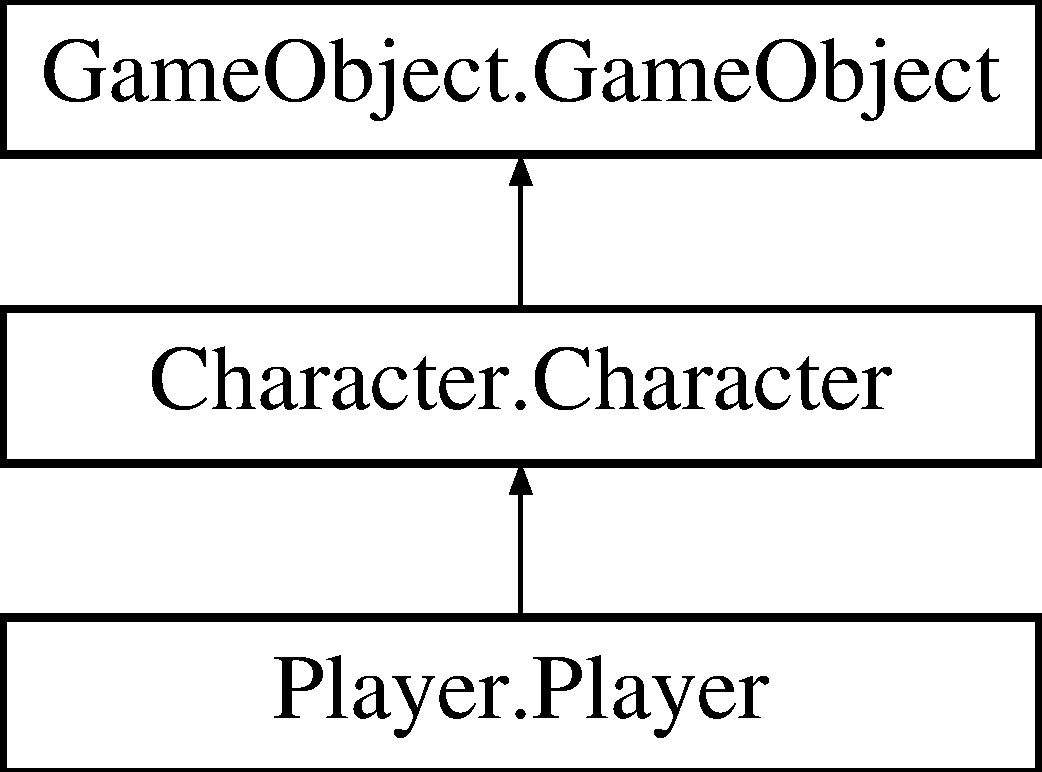
\includegraphics[height=3.000000cm]{classCharacter_1_1Character}
\end{center}
\end{figure}
\subsection*{\-Public \-Member \-Functions}
\begin{DoxyCompactItemize}
\item 
def \hyperlink{classCharacter_1_1Character_aaeea994d98f7e7d51dccdfdcb06dbd73}{\-\_\-\-\_\-init\-\_\-\-\_\-}
\item 
def \hyperlink{classCharacter_1_1Character_a30b2039d08a858e628f1801260fa5542}{introduction}
\item 
def \hyperlink{classCharacter_1_1Character_a0c749b4e77403ff141f30bc9dc22521b}{catching\-Up}
\end{DoxyCompactItemize}
\subsection*{\-Public \-Attributes}
\begin{DoxyCompactItemize}
\item 
\hypertarget{classCharacter_1_1Character_ac7d72676b39b540d595e2dd1e24a81a3}{\hyperlink{classCharacter_1_1Character_ac7d72676b39b540d595e2dd1e24a81a3}{velocity}}\label{classCharacter_1_1Character_ac7d72676b39b540d595e2dd1e24a81a3}

\begin{DoxyCompactList}\small\item\em \-A 3\-D vector for the \hyperlink{classCharacter_1_1Character}{\-Character}'s velocity. \end{DoxyCompactList}\item 
\hypertarget{classCharacter_1_1Character_afe735ef35ec0f469fea8276d83780bf6}{\hyperlink{classCharacter_1_1Character_afe735ef35ec0f469fea8276d83780bf6}{acceleration}}\label{classCharacter_1_1Character_afe735ef35ec0f469fea8276d83780bf6}

\begin{DoxyCompactList}\small\item\em \-A 3\-D vector for the \hyperlink{classCharacter_1_1Character}{\-Character}'s acceleration. \end{DoxyCompactList}\end{DoxyCompactItemize}


\subsection{\-Detailed \-Description}
\begin{DoxyVerb}A GameObject that can move in space and have a behaviour. player or NPC\end{DoxyVerb}
 

\subsection{\-Constructor \& \-Destructor \-Documentation}
\hypertarget{classCharacter_1_1Character_aaeea994d98f7e7d51dccdfdcb06dbd73}{\index{\-Character\-::\-Character@{\-Character\-::\-Character}!\-\_\-\-\_\-init\-\_\-\-\_\-@{\-\_\-\-\_\-init\-\_\-\-\_\-}}
\index{\-\_\-\-\_\-init\-\_\-\-\_\-@{\-\_\-\-\_\-init\-\_\-\-\_\-}!Character::Character@{\-Character\-::\-Character}}
\subsubsection[{\-\_\-\-\_\-init\-\_\-\-\_\-}]{\setlength{\rightskip}{0pt plus 5cm}def {\bf \-Character.\-Character.\-\_\-\-\_\-init\-\_\-\-\_\-} (
\begin{DoxyParamCaption}
\item[{}]{self, }
\item[{}]{objid, }
\item[{}]{position, }
\item[{}]{gridposition, }
\item[{}]{rotation, }
\item[{}]{scale, }
\item[{}]{lookat, }
\item[{}]{tags, }
\item[{}]{visibility, }
\item[{}]{interactability, }
\item[{}]{interactiondomain, }
\item[{}]{v0, }
\item[{}]{a0, }
\item[{}]{isrigid = {\ttfamily \-False}, }
\item[{}]{parent = {\ttfamily \-None}, }
\item[{}]{layer = {\ttfamily \-None}, }
\item[{}]{interactiontimelimit = {\ttfamily 0}, }
\item[{}]{script = {\ttfamily \-None}, }
\item[{}]{team = {\ttfamily \-None}, }
\item[{}]{latency = {\ttfamily 0}, }
\item[{}]{score = {\ttfamily 0}}
\end{DoxyParamCaption}
)}}\label{classCharacter_1_1Character_aaeea994d98f7e7d51dccdfdcb06dbd73}
\begin{DoxyVerb}Character.__init__(self,
 objid,
 position,
 gridposition,
 rotation,
 scale,
 lookat,
 tags,
 visibility,
 interactability,
 interactiondomain,
 
 v0,
 a0,
                  
 isrigid = False,
 parent = None,
 layer = None,
 interactiontimelimit = 0,
 script = None,
 team = None,
 latency  = 0,
 score = 0
)
Initialization function for a Character. All arguments except v0 and a0
are documented on GameObject class

v0 is a 3D vector of the object's initial velocity
a0 is a 3D vector of the object's initial acceleration
\end{DoxyVerb}
 

\subsection{\-Member \-Function \-Documentation}
\hypertarget{classCharacter_1_1Character_a0c749b4e77403ff141f30bc9dc22521b}{\index{\-Character\-::\-Character@{\-Character\-::\-Character}!catching\-Up@{catching\-Up}}
\index{catching\-Up@{catching\-Up}!Character::Character@{\-Character\-::\-Character}}
\subsubsection[{catching\-Up}]{\setlength{\rightskip}{0pt plus 5cm}def {\bf \-Character.\-Character.\-catching\-Up} (
\begin{DoxyParamCaption}
\item[{}]{self}
\end{DoxyParamCaption}
)}}\label{classCharacter_1_1Character_a0c749b4e77403ff141f30bc9dc22521b}
\begin{DoxyVerb}Generates a JSON friendly dictionary with
all the object's attributes and values.
This function is intended as a update on the object's state,
sent to receivers that are already able to identify the object.
\end{DoxyVerb}
 

\-Reimplemented from \hyperlink{classGameObject_1_1GameObject_a86432a4b5f554dc490504b7ca01e2cb9}{\-Game\-Object.\-Game\-Object}.

\hypertarget{classCharacter_1_1Character_a30b2039d08a858e628f1801260fa5542}{\index{\-Character\-::\-Character@{\-Character\-::\-Character}!introduction@{introduction}}
\index{introduction@{introduction}!Character::Character@{\-Character\-::\-Character}}
\subsubsection[{introduction}]{\setlength{\rightskip}{0pt plus 5cm}def {\bf \-Character.\-Character.\-introduction} (
\begin{DoxyParamCaption}
\item[{}]{self}
\end{DoxyParamCaption}
)}}\label{classCharacter_1_1Character_a30b2039d08a858e628f1801260fa5542}
\begin{DoxyVerb}Generates a JSON friendly dictionary with
all the object's attributes and values.
This function is intended as a first introduction of the object,
to receivers that are unaware of its existence.
\end{DoxyVerb}
 

\-Reimplemented from \hyperlink{classGameObject_1_1GameObject_a10826507bf158f9678071a3eddcee0e9}{\-Game\-Object.\-Game\-Object}.



\-The documentation for this class was generated from the following file\-:\begin{DoxyCompactItemize}
\item 
\-Character.\-py\end{DoxyCompactItemize}

\hypertarget{classCollision_1_1Collision}{\section{\-Collision.\-Collision \-Class \-Reference}
\label{classCollision_1_1Collision}\index{\-Collision.\-Collision@{\-Collision.\-Collision}}
}
\subsection*{\-Public \-Member \-Functions}
\begin{DoxyCompactItemize}
\item 
def \hyperlink{classCollision_1_1Collision_a4acfcbd4a12cc49011e1565f4f4d4d84}{\-\_\-\-\_\-init\-\_\-\-\_\-}
\item 
def \hyperlink{classCollision_1_1Collision_a3d88b2d02247db3b7009b0674e249fee}{introduction}
\item 
def \hyperlink{classCollision_1_1Collision_a0d785c437c39344795e22413e14c486c}{catching\-Up}
\end{DoxyCompactItemize}
\subsection*{\-Public \-Attributes}
\begin{DoxyCompactItemize}
\item 
\hypertarget{classCollision_1_1Collision_ad0bf12b64094d6d47eebd2f09c14daed}{\hyperlink{classCollision_1_1Collision_ad0bf12b64094d6d47eebd2f09c14daed}{culprit}}\label{classCollision_1_1Collision_ad0bf12b64094d6d47eebd2f09c14daed}

\begin{DoxyCompactList}\small\item\em \-The first object involved in the collision. \end{DoxyCompactList}\item 
\hypertarget{classCollision_1_1Collision_ae9b952cce23fa8dcc4dcaf3c10db8332}{\hyperlink{classCollision_1_1Collision_ae9b952cce23fa8dcc4dcaf3c10db8332}{victim}}\label{classCollision_1_1Collision_ae9b952cce23fa8dcc4dcaf3c10db8332}

\begin{DoxyCompactList}\small\item\em \-The second object involved in the collision. \end{DoxyCompactList}\item 
\hypertarget{classCollision_1_1Collision_a01d99d59d7e43d843c90e40413878105}{\hyperlink{classCollision_1_1Collision_a01d99d59d7e43d843c90e40413878105}{turn}}\label{classCollision_1_1Collision_a01d99d59d7e43d843c90e40413878105}

\begin{DoxyCompactList}\small\item\em \-The \-Number of the turn in which the collision occured. \end{DoxyCompactList}\end{DoxyCompactItemize}


\subsection{\-Constructor \& \-Destructor \-Documentation}
\hypertarget{classCollision_1_1Collision_a4acfcbd4a12cc49011e1565f4f4d4d84}{\index{\-Collision\-::\-Collision@{\-Collision\-::\-Collision}!\-\_\-\-\_\-init\-\_\-\-\_\-@{\-\_\-\-\_\-init\-\_\-\-\_\-}}
\index{\-\_\-\-\_\-init\-\_\-\-\_\-@{\-\_\-\-\_\-init\-\_\-\-\_\-}!Collision::Collision@{\-Collision\-::\-Collision}}
\subsubsection[{\-\_\-\-\_\-init\-\_\-\-\_\-}]{\setlength{\rightskip}{0pt plus 5cm}def {\bf \-Collision.\-Collision.\-\_\-\-\_\-init\-\_\-\-\_\-} (
\begin{DoxyParamCaption}
\item[{}]{self, }
\item[{}]{culprit, }
\item[{}]{victim, }
\item[{}]{turn}
\end{DoxyParamCaption}
)}}\label{classCollision_1_1Collision_a4acfcbd4a12cc49011e1565f4f4d4d84}
\begin{DoxyVerb}Collision.__init__(self, obj1, obj2)
initialization for Collision object.

culprit and victim are the two objects involved in the collision
turn is the turn number on which the collision occured\end{DoxyVerb}
 

\subsection{\-Member \-Function \-Documentation}
\hypertarget{classCollision_1_1Collision_a0d785c437c39344795e22413e14c486c}{\index{\-Collision\-::\-Collision@{\-Collision\-::\-Collision}!catching\-Up@{catching\-Up}}
\index{catching\-Up@{catching\-Up}!Collision::Collision@{\-Collision\-::\-Collision}}
\subsubsection[{catching\-Up}]{\setlength{\rightskip}{0pt plus 5cm}def {\bf \-Collision.\-Collision.\-catching\-Up} (
\begin{DoxyParamCaption}
\item[{}]{self}
\end{DoxyParamCaption}
)}}\label{classCollision_1_1Collision_a0d785c437c39344795e22413e14c486c}
\begin{DoxyVerb}Generates a JSON friendly dictionary with
all the object's attributes and values.
This function is intended as a update on the object's state,
sent to receivers that are already able to identify the object.
\end{DoxyVerb}
 \hypertarget{classCollision_1_1Collision_a3d88b2d02247db3b7009b0674e249fee}{\index{\-Collision\-::\-Collision@{\-Collision\-::\-Collision}!introduction@{introduction}}
\index{introduction@{introduction}!Collision::Collision@{\-Collision\-::\-Collision}}
\subsubsection[{introduction}]{\setlength{\rightskip}{0pt plus 5cm}def {\bf \-Collision.\-Collision.\-introduction} (
\begin{DoxyParamCaption}
\item[{}]{self}
\end{DoxyParamCaption}
)}}\label{classCollision_1_1Collision_a3d88b2d02247db3b7009b0674e249fee}
\begin{DoxyVerb}Generates a JSON friendly dictionary with
all the object's attributes and values.
This function is intended as a first introduction of the object,
to receivers that are unaware of its existence.
\end{DoxyVerb}
 

\-The documentation for this class was generated from the following file\-:\begin{DoxyCompactItemize}
\item 
\-Collision.\-py\end{DoxyCompactItemize}

\hypertarget{classGame_1_1Game}{\section{\-Game.\-Game \-Class \-Reference}
\label{classGame_1_1Game}\index{\-Game.\-Game@{\-Game.\-Game}}
}
\subsection*{\-Public \-Member \-Functions}
\begin{DoxyCompactItemize}
\item 
def \hyperlink{classGame_1_1Game_a527f0ebbb5bce3e8cdfc3d4ff8a983a5}{\-\_\-\-\_\-init\-\_\-\-\_\-}
\item 
def \hyperlink{classGame_1_1Game_a37248ca770739409b6517ae924a4e4e7}{run}
\item 
def \hyperlink{classGame_1_1Game_add568019cd768b7acb98ab0c71d43393}{add\-Poll}
\item 
def \hyperlink{classGame_1_1Game_a202b94dcc6ea36d44e2b9c8848d3360b}{switch\-Off\-Poll}
\item 
def \hyperlink{classGame_1_1Game_af7ebb81ec3b8969e3dc3ae42d8446b57}{switch\-On\-Poll}
\item 
def \hyperlink{classGame_1_1Game_a9ca82128ce923d5eed173141459d70eb}{initial\-State}
\item 
def \hyperlink{classGame_1_1Game_a830019e0641847c416a2c4adfae8f43e}{current\-State}
\item 
def \hyperlink{classGame_1_1Game_a4f05d65d609b8772d3a0e01b2b6b56e1}{push\-State}
\item 
def \hyperlink{classGame_1_1Game_aa6154ca487348bae42564ff00675f0fb}{current\-State\-Diff}
\end{DoxyCompactItemize}
\subsection*{\-Public \-Attributes}
\begin{DoxyCompactItemize}
\item 
\hypertarget{classGame_1_1Game_a22c0db7acba3af745d60b16b997e9439}{\hyperlink{classGame_1_1Game_a22c0db7acba3af745d60b16b997e9439}{name}}\label{classGame_1_1Game_a22c0db7acba3af745d60b16b997e9439}

\begin{DoxyCompactList}\small\item\em \-The \hyperlink{classGame_1_1Game}{\-Game}'s name. \end{DoxyCompactList}\item 
\hypertarget{classGame_1_1Game_acdc29dd60a3b80f3dd6d9c6a069e551d}{\hyperlink{classGame_1_1Game_acdc29dd60a3b80f3dd6d9c6a069e551d}{description}}\label{classGame_1_1Game_acdc29dd60a3b80f3dd6d9c6a069e551d}

\begin{DoxyCompactList}\small\item\em \-The \hyperlink{classGame_1_1Game}{\-Game}'s description. \end{DoxyCompactList}\item 
\hypertarget{classGame_1_1Game_a17f9756d1c7683b98d8c3b42b2cd42bd}{\hyperlink{classGame_1_1Game_a17f9756d1c7683b98d8c3b42b2cd42bd}{space}}\label{classGame_1_1Game_a17f9756d1c7683b98d8c3b42b2cd42bd}

\begin{DoxyCompactList}\small\item\em \hyperlink{classGame_1_1Game}{\-Game}'s \-Game\-Space object. \end{DoxyCompactList}\item 
\hypertarget{classGame_1_1Game_a5c4c51b255ba66dcbc0eb1c689e9f97d}{\hyperlink{classGame_1_1Game_a5c4c51b255ba66dcbc0eb1c689e9f97d}{gameobjects}}\label{classGame_1_1Game_a5c4c51b255ba66dcbc0eb1c689e9f97d}

\begin{DoxyCompactList}\small\item\em \-The \hyperlink{classGame_1_1Game}{\-Game}'s list of \-Game\-Objects (\hyperlink{namespaceGameObject}{\-Game\-Object}) \end{DoxyCompactList}\item 
\hypertarget{classGame_1_1Game_ac616645ae9beaf693c3be58daea72665}{\hyperlink{classGame_1_1Game_ac616645ae9beaf693c3be58daea72665}{teams}}\label{classGame_1_1Game_ac616645ae9beaf693c3be58daea72665}

\begin{DoxyCompactList}\small\item\em \-The \hyperlink{classGame_1_1Game}{\-Game}'s list of \-Teams (\hyperlink{namespaceTeam}{\-Team}) \end{DoxyCompactList}\item 
\hypertarget{classGame_1_1Game_ae533135b459d1563769361e0022af7da}{\hyperlink{classGame_1_1Game_ae533135b459d1563769361e0022af7da}{isdiscrete}}\label{classGame_1_1Game_ae533135b459d1563769361e0022af7da}

\begin{DoxyCompactList}\small\item\em \-Boolean to indicate whether or not the to use self.\-space.\-grid for objects position. \end{DoxyCompactList}\item 
\hypertarget{classGame_1_1Game_ab9913d7afe86cddc153b9a299823dcb2}{\hyperlink{classGame_1_1Game_ab9913d7afe86cddc153b9a299823dcb2}{polls}}\label{classGame_1_1Game_ab9913d7afe86cddc153b9a299823dcb2}

\begin{DoxyCompactList}\small\item\em \-A list of \-Polls (\hyperlink{classGame_1_1Poll}{\-Poll}) \end{DoxyCompactList}\item 
\hypertarget{classGame_1_1Game_a6e7630196dde4954d8915a58a1557b00}{\hyperlink{classGame_1_1Game_a6e7630196dde4954d8915a58a1557b00}{activepolls}}\label{classGame_1_1Game_a6e7630196dde4954d8915a58a1557b00}

\begin{DoxyCompactList}\small\item\em \-The subset of active \-Polls (\hyperlink{classGame_1_1Poll}{\-Poll}) within self.\-polls. \end{DoxyCompactList}\item 
\hypertarget{classGame_1_1Game_ae8fd4be17b48fb5a5d68146cb092e4fb}{\hyperlink{classGame_1_1Game_ae8fd4be17b48fb5a5d68146cb092e4fb}{finit}}\label{classGame_1_1Game_ae8fd4be17b48fb5a5d68146cb092e4fb}

\begin{DoxyCompactList}\small\item\em \-The \hyperlink{classGame_1_1Game}{\-Game}'s initialization function. \end{DoxyCompactList}\item 
\hypertarget{classGame_1_1Game_ad0fa73cb5206c668d9916ea6e4d50478}{\hyperlink{classGame_1_1Game_ad0fa73cb5206c668d9916ea6e4d50478}{fturn}}\label{classGame_1_1Game_ad0fa73cb5206c668d9916ea6e4d50478}

\begin{DoxyCompactList}\small\item\em \-A function to be called on each new turn. \end{DoxyCompactList}\item 
\hypertarget{classGame_1_1Game_ad2b03faf4ed27993323f19a97d70ca4c}{\hyperlink{classGame_1_1Game_ad2b03faf4ed27993323f19a97d70ca4c}{fend}}\label{classGame_1_1Game_ad2b03faf4ed27993323f19a97d70ca4c}

\begin{DoxyCompactList}\small\item\em \-A function to be called when the game ends. \end{DoxyCompactList}\item 
\hypertarget{classGame_1_1Game_ac71449b283ea63a19f06872b38c2b655}{\hyperlink{classGame_1_1Game_ac71449b283ea63a19f06872b38c2b655}{lastturn}}\label{classGame_1_1Game_ac71449b283ea63a19f06872b38c2b655}

\begin{DoxyCompactList}\small\item\em \-A boolean that inidicates if the \hyperlink{classGame_1_1Game}{\-Game}'s current turn is its last. \end{DoxyCompactList}\item 
\hypertarget{classGame_1_1Game_abae9b3fda20fe7019193febded78b39d}{\hyperlink{classGame_1_1Game_abae9b3fda20fe7019193febded78b39d}{turncount}}\label{classGame_1_1Game_abae9b3fda20fe7019193febded78b39d}

\begin{DoxyCompactList}\small\item\em \-The number of the current turn. \end{DoxyCompactList}\item 
\hypertarget{classGame_1_1Game_a2aef6fc5c75fc51ee1106c9fad77883e}{\hyperlink{classGame_1_1Game_a2aef6fc5c75fc51ee1106c9fad77883e}{rigidobjects}}\label{classGame_1_1Game_a2aef6fc5c75fc51ee1106c9fad77883e}

\begin{DoxyCompactList}\small\item\em \-A subset of rigid \-Game\-Objects (\hyperlink{namespaceGameObject}{\-Game\-Object}) within self.\-gameobjects. \end{DoxyCompactList}\item 
\hypertarget{classGame_1_1Game_a8ccce12618221590a9732debd751e2d2}{\hyperlink{classGame_1_1Game_a8ccce12618221590a9732debd751e2d2}{collisions}}\label{classGame_1_1Game_a8ccce12618221590a9732debd751e2d2}

\begin{DoxyCompactList}\small\item\em \-A list of collisions (\-Collision) to be addressed. \end{DoxyCompactList}\item 
\hypertarget{classGame_1_1Game_a98127da75f494b585a5ee33f99c75823}{\hyperlink{classGame_1_1Game_a98127da75f494b585a5ee33f99c75823}{statebuff}}\label{classGame_1_1Game_a98127da75f494b585a5ee33f99c75823}

\begin{DoxyCompactList}\small\item\em \-A list of past game states self.\-paststates\mbox{[}0\mbox{]} is the current state self.\-paststates\mbox{[}n\mbox{]} is the n'th past state. \end{DoxyCompactList}\end{DoxyCompactItemize}
\subsection*{\-Static \-Public \-Attributes}
\begin{DoxyCompactItemize}
\item 
\hypertarget{classGame_1_1Game_a71a6e20de6b0164b8262d44ba73449e6}{\hyperlink{classGame_1_1Game_a71a6e20de6b0164b8262d44ba73449e6}{initialstate} = \-None}\label{classGame_1_1Game_a71a6e20de6b0164b8262d44ba73449e6}

\begin{DoxyCompactList}\small\item\em \-The dictionary containing the \hyperlink{classGame_1_1Game}{\-Game}'s initial state information. \end{DoxyCompactList}\end{DoxyCompactItemize}


\subsection{\-Detailed \-Description}
\begin{DoxyVerb}The Class that contains the game itself.
It has the game's state and is responsible for its execution
\end{DoxyVerb}
 

\subsection{\-Constructor \& \-Destructor \-Documentation}
\hypertarget{classGame_1_1Game_a527f0ebbb5bce3e8cdfc3d4ff8a983a5}{\index{\-Game\-::\-Game@{\-Game\-::\-Game}!\-\_\-\-\_\-init\-\_\-\-\_\-@{\-\_\-\-\_\-init\-\_\-\-\_\-}}
\index{\-\_\-\-\_\-init\-\_\-\-\_\-@{\-\_\-\-\_\-init\-\_\-\-\_\-}!Game::Game@{\-Game\-::\-Game}}
\subsubsection[{\-\_\-\-\_\-init\-\_\-\-\_\-}]{\setlength{\rightskip}{0pt plus 5cm}def {\bf \-Game.\-Game.\-\_\-\-\_\-init\-\_\-\-\_\-} (
\begin{DoxyParamCaption}
\item[{}]{self, }
\item[{}]{name, }
\item[{}]{description, }
\item[{}]{space, }
\item[{}]{gameobjects, }
\item[{}]{teams, }
\item[{}]{isdiscrete, }
\item[{}]{polls, }
\item[{}]{finit = {\ttfamily lambda~x\-:~\-None}, }
\item[{}]{fturn = {\ttfamily lambda~x\-:~\-None}, }
\item[{}]{fend = {\ttfamily lambda~x\-:~\-None}, }
\item[{}]{statebuffsize = {\ttfamily 2}}
\end{DoxyParamCaption}
)}}\label{classGame_1_1Game_a527f0ebbb5bce3e8cdfc3d4ff8a983a5}
\begin{DoxyVerb}Game.__init__(self,
      name,
      description,
      gameobjects,
      teams,
      
      finit = lambda: None,
      fturn = lambda: None,
      fend = lambda: None,
      statebuffsize = 2
     )
     
name is the Game's name

description is a brief Game description

space is the Game's GameSpace

gameobjects is a list of the Game's GameObjects

teams is a list of the Game's Teams

isdiscrete indicates if the game space is discrete.
If so, all objects will be positioned according to space's Grid Cells

finit is a function to be called once

fturn is a function that marks de division between Game turns

fend is a function to be called once right before the Game ends

statebuffsize is the size of the states buffer, or how many turns previous
to current are stored
\end{DoxyVerb}
 

\subsection{\-Member \-Function \-Documentation}
\hypertarget{classGame_1_1Game_add568019cd768b7acb98ab0c71d43393}{\index{\-Game\-::\-Game@{\-Game\-::\-Game}!add\-Poll@{add\-Poll}}
\index{add\-Poll@{add\-Poll}!Game::Game@{\-Game\-::\-Game}}
\subsubsection[{add\-Poll}]{\setlength{\rightskip}{0pt plus 5cm}def {\bf \-Game.\-Game.\-add\-Poll} (
\begin{DoxyParamCaption}
\item[{}]{self, }
\item[{}]{poll}
\end{DoxyParamCaption}
)}}\label{classGame_1_1Game_add568019cd768b7acb98ab0c71d43393}
\begin{DoxyVerb}Game.addPoll(self, poll)
A function to add a Poll to a Game.
Returns True on success and False on failure
\end{DoxyVerb}
 \hypertarget{classGame_1_1Game_a830019e0641847c416a2c4adfae8f43e}{\index{\-Game\-::\-Game@{\-Game\-::\-Game}!current\-State@{current\-State}}
\index{current\-State@{current\-State}!Game::Game@{\-Game\-::\-Game}}
\subsubsection[{current\-State}]{\setlength{\rightskip}{0pt plus 5cm}def {\bf \-Game.\-Game.\-current\-State} (
\begin{DoxyParamCaption}
\item[{}]{self}
\end{DoxyParamCaption}
)}}\label{classGame_1_1Game_a830019e0641847c416a2c4adfae8f43e}
\begin{DoxyVerb}Game.currentState(self)
Returns a dictionary containing the Game's current state
\end{DoxyVerb}
 \hypertarget{classGame_1_1Game_aa6154ca487348bae42564ff00675f0fb}{\index{\-Game\-::\-Game@{\-Game\-::\-Game}!current\-State\-Diff@{current\-State\-Diff}}
\index{current\-State\-Diff@{current\-State\-Diff}!Game::Game@{\-Game\-::\-Game}}
\subsubsection[{current\-State\-Diff}]{\setlength{\rightskip}{0pt plus 5cm}def {\bf \-Game.\-Game.\-current\-State\-Diff} (
\begin{DoxyParamCaption}
\item[{}]{self, }
\item[{}]{i = {\ttfamily 0}, }
\item[{}]{j = {\ttfamily 1}}
\end{DoxyParamCaption}
)}}\label{classGame_1_1Game_aa6154ca487348bae42564ff00675f0fb}
\begin{DoxyVerb}Game.currentStateDiff(self)
Returns a minimal dictionary containing only the differences between
self.statebuff[i] and self.statebuff[j]. Any object with access to the Game's
last state can deduce its current state by the differences.
This function is used to minimize the network's communication
overhead.
\end{DoxyVerb}
 \hypertarget{classGame_1_1Game_a9ca82128ce923d5eed173141459d70eb}{\index{\-Game\-::\-Game@{\-Game\-::\-Game}!initial\-State@{initial\-State}}
\index{initial\-State@{initial\-State}!Game::Game@{\-Game\-::\-Game}}
\subsubsection[{initial\-State}]{\setlength{\rightskip}{0pt plus 5cm}def {\bf \-Game.\-Game.\-initial\-State} (
\begin{DoxyParamCaption}
\item[{}]{self}
\end{DoxyParamCaption}
)}}\label{classGame_1_1Game_a9ca82128ce923d5eed173141459d70eb}
\begin{DoxyVerb}Game.initialState(self)
Returns a dictionary containg the game initial state
and sets static Game.initialstate
\end{DoxyVerb}
 \hypertarget{classGame_1_1Game_a4f05d65d609b8772d3a0e01b2b6b56e1}{\index{\-Game\-::\-Game@{\-Game\-::\-Game}!push\-State@{push\-State}}
\index{push\-State@{push\-State}!Game::Game@{\-Game\-::\-Game}}
\subsubsection[{push\-State}]{\setlength{\rightskip}{0pt plus 5cm}def {\bf \-Game.\-Game.\-push\-State} (
\begin{DoxyParamCaption}
\item[{}]{self, }
\item[{}]{state}
\end{DoxyParamCaption}
)}}\label{classGame_1_1Game_a4f05d65d609b8772d3a0e01b2b6b56e1}
\begin{DoxyVerb}Game.pushState(self)
adds the argument to self.statebuff
\end{DoxyVerb}
 \hypertarget{classGame_1_1Game_a37248ca770739409b6517ae924a4e4e7}{\index{\-Game\-::\-Game@{\-Game\-::\-Game}!run@{run}}
\index{run@{run}!Game::Game@{\-Game\-::\-Game}}
\subsubsection[{run}]{\setlength{\rightskip}{0pt plus 5cm}def {\bf \-Game.\-Game.\-run} (
\begin{DoxyParamCaption}
\item[{}]{self}
\end{DoxyParamCaption}
)}}\label{classGame_1_1Game_a37248ca770739409b6517ae924a4e4e7}
\begin{DoxyVerb}Game.run(self)
the Game's execution function
\end{DoxyVerb}
 \hypertarget{classGame_1_1Game_a202b94dcc6ea36d44e2b9c8848d3360b}{\index{\-Game\-::\-Game@{\-Game\-::\-Game}!switch\-Off\-Poll@{switch\-Off\-Poll}}
\index{switch\-Off\-Poll@{switch\-Off\-Poll}!Game::Game@{\-Game\-::\-Game}}
\subsubsection[{switch\-Off\-Poll}]{\setlength{\rightskip}{0pt plus 5cm}def {\bf \-Game.\-Game.\-switch\-Off\-Poll} (
\begin{DoxyParamCaption}
\item[{}]{self, }
\item[{}]{poll}
\end{DoxyParamCaption}
)}}\label{classGame_1_1Game_a202b94dcc6ea36d44e2b9c8848d3360b}
\begin{DoxyVerb}Game.switchOffPoll(self, poll)
Function to make an active Poll inactive.
Returns True on success and False on failure
\end{DoxyVerb}
 \hypertarget{classGame_1_1Game_af7ebb81ec3b8969e3dc3ae42d8446b57}{\index{\-Game\-::\-Game@{\-Game\-::\-Game}!switch\-On\-Poll@{switch\-On\-Poll}}
\index{switch\-On\-Poll@{switch\-On\-Poll}!Game::Game@{\-Game\-::\-Game}}
\subsubsection[{switch\-On\-Poll}]{\setlength{\rightskip}{0pt plus 5cm}def {\bf \-Game.\-Game.\-switch\-On\-Poll} (
\begin{DoxyParamCaption}
\item[{}]{self, }
\item[{}]{poll}
\end{DoxyParamCaption}
)}}\label{classGame_1_1Game_af7ebb81ec3b8969e3dc3ae42d8446b57}
\begin{DoxyVerb}Game.switchOnPoll(self, poll)
Function to make an inactive Poll active.
Returns True on success and False on failure
\end{DoxyVerb}
 

\-The documentation for this class was generated from the following file\-:\begin{DoxyCompactItemize}
\item 
\-Game.\-py\end{DoxyCompactItemize}

\hypertarget{classGameObject_1_1GameObject}{\section{\-Game\-Object.\-Game\-Object \-Class \-Reference}
\label{classGameObject_1_1GameObject}\index{\-Game\-Object.\-Game\-Object@{\-Game\-Object.\-Game\-Object}}
}
\-Inheritance diagram for \-Game\-Object.\-Game\-Object\-:\begin{figure}[H]
\begin{center}
\leavevmode
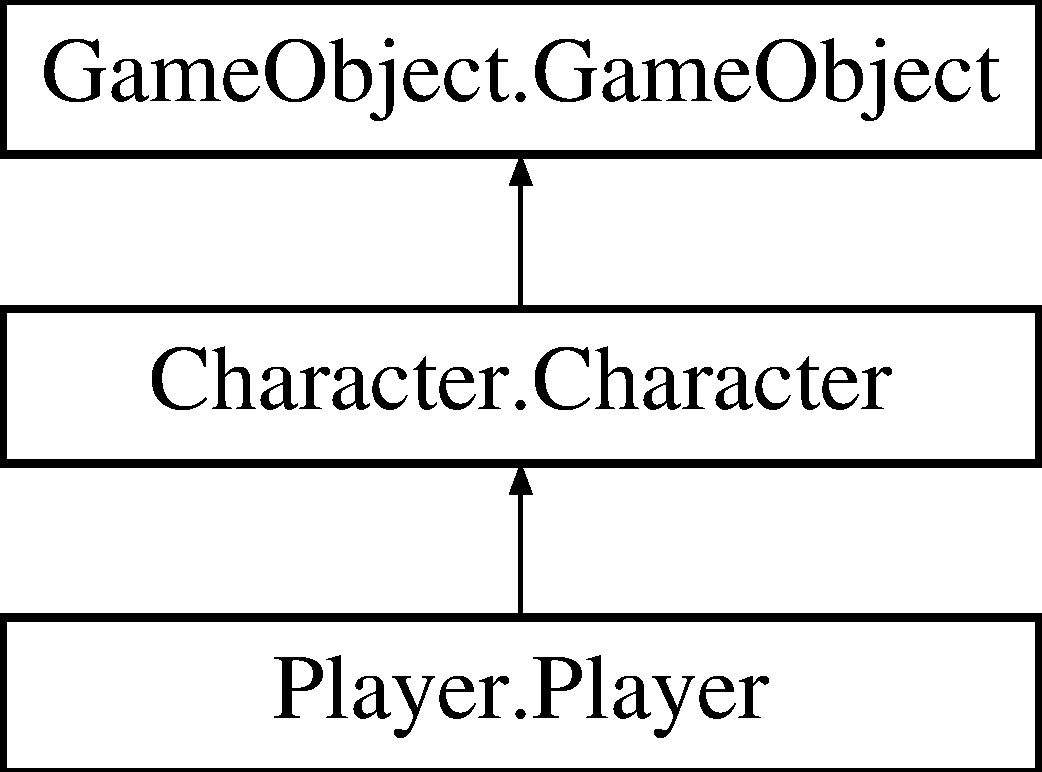
\includegraphics[height=3.000000cm]{classGameObject_1_1GameObject}
\end{center}
\end{figure}
\subsection*{\-Public \-Member \-Functions}
\begin{DoxyCompactItemize}
\item 
def \hyperlink{classGameObject_1_1GameObject_a388f494ea5093578fa2a386b20eb9f4a}{\-\_\-\-\_\-init\-\_\-\-\_\-}
\item 
def \hyperlink{classGameObject_1_1GameObject_a7cb3c8e68eea9ec7a18aa5f12c49299f}{add\-Interaction}
\item 
def \hyperlink{classGameObject_1_1GameObject_a12165afe9211fd3a2d0e52cf5a364bec}{add\-Tags}
\item 
def \hyperlink{classGameObject_1_1GameObject_aca961c48562553b68319583a74fb3327}{remove\-Tags}
\item 
def \hyperlink{classGameObject_1_1GameObject_af03461727168ab632690aaf710c0f2bd}{get\-Super\-Class\-Name}
\item 
def \hyperlink{classGameObject_1_1GameObject_a10826507bf158f9678071a3eddcee0e9}{introduction}
\item 
def \hyperlink{classGameObject_1_1GameObject_a86432a4b5f554dc490504b7ca01e2cb9}{catching\-Up}
\end{DoxyCompactItemize}
\subsection*{\-Static \-Public \-Member \-Functions}
\begin{DoxyCompactItemize}
\item 
def \hyperlink{classGameObject_1_1GameObject_abea66e6f349308e235a6f044a1276f4b}{init\-Tag\-Domain}
\item 
def \hyperlink{classGameObject_1_1GameObject_aa37db10065043a169cccbe7d3a3fda92}{obj\-From\-Id}
\item 
def \hyperlink{classGameObject_1_1GameObject_a114c8b7fd3c2f7450b07b796fc982ea6}{id\-From\-Obj}
\end{DoxyCompactItemize}
\subsection*{\-Public \-Attributes}
\begin{DoxyCompactItemize}
\item 
\hyperlink{classGameObject_1_1GameObject_ac9ae5ed4d040061ff584751e20799a7a}{objid}
\begin{DoxyCompactList}\small\item\em \-A \hyperlink{classGameObject_1_1GameObject}{\-Game\-Object}'s unique identifier. \end{DoxyCompactList}\item 
\hyperlink{classGameObject_1_1GameObject_aa496066be50cb5918bc7cbf56d14cf7a}{parent}
\begin{DoxyCompactList}\small\item\em \-A \hyperlink{classGameObject_1_1GameObject}{\-Game\-Object}'s parent. \end{DoxyCompactList}\item 
\hypertarget{classGameObject_1_1GameObject_aef72ecd07ce7acb7245f42dd7f307c04}{\hyperlink{classGameObject_1_1GameObject_aef72ecd07ce7acb7245f42dd7f307c04}{layer}}\label{classGameObject_1_1GameObject_aef72ecd07ce7acb7245f42dd7f307c04}

\begin{DoxyCompactList}\small\item\em \-The \hyperlink{classGameObject_1_1Layer}{\-Layer} to which the \hyperlink{classGameObject_1_1GameObject}{\-Game\-Object} belongs. \end{DoxyCompactList}\item 
\hypertarget{classGameObject_1_1GameObject_a77b43e6eb78d01f16bb5b098d62d53d4}{\hyperlink{classGameObject_1_1GameObject_a77b43e6eb78d01f16bb5b098d62d53d4}{tags}}\label{classGameObject_1_1GameObject_a77b43e6eb78d01f16bb5b098d62d53d4}

\begin{DoxyCompactList}\small\item\em \-A list of tags (a subset of \-Game\-Object.\-tagdomain) \end{DoxyCompactList}\item 
\hypertarget{classGameObject_1_1GameObject_a39bf412c9900083432b58f2dbbe1d5fb}{\hyperlink{classGameObject_1_1GameObject_a39bf412c9900083432b58f2dbbe1d5fb}{visibility}}\label{classGameObject_1_1GameObject_a39bf412c9900083432b58f2dbbe1d5fb}

\begin{DoxyCompactList}\small\item\em \-A list of \-Game\-Objects allowed to see the \hyperlink{classGameObject_1_1GameObject}{\-Game\-Object} \-Implementation of visibility is left to the game developer. \end{DoxyCompactList}\item 
\hypertarget{classGameObject_1_1GameObject_aa48d265929b12d794a9ac630046b74cf}{\hyperlink{classGameObject_1_1GameObject_aa48d265929b12d794a9ac630046b74cf}{interactability}}\label{classGameObject_1_1GameObject_aa48d265929b12d794a9ac630046b74cf}

\begin{DoxyCompactList}\small\item\em \-A list of \-Game\-Objects allowed to interact with the \hyperlink{classGameObject_1_1GameObject}{\-Game\-Object} \-Implementation of interactability is left to the game developer. \end{DoxyCompactList}\item 
\hypertarget{classGameObject_1_1GameObject_a2c3d51c7d53086f093ba84dcd0b12611}{\hyperlink{classGameObject_1_1GameObject_a2c3d51c7d53086f093ba84dcd0b12611}{position}}\label{classGameObject_1_1GameObject_a2c3d51c7d53086f093ba84dcd0b12611}

\begin{DoxyCompactList}\small\item\em \-A 3\-D vector with the \hyperlink{classGameObject_1_1GameObject}{\-Game\-Object}'s spacial position relative to self.\-parent. \end{DoxyCompactList}\item 
\hypertarget{classGameObject_1_1GameObject_a20ee6e5619e5bda604667f3c5427302f}{\hyperlink{classGameObject_1_1GameObject_a20ee6e5619e5bda604667f3c5427302f}{space}}\label{classGameObject_1_1GameObject_a20ee6e5619e5bda604667f3c5427302f}

\begin{DoxyCompactList}\small\item\em \-A \-Game\-Space object to which all of the \hyperlink{classGameObject_1_1GameObject}{\-Game\-Object} spatial information refers. \end{DoxyCompactList}\item 
\hypertarget{classGameObject_1_1GameObject_ae6912b906836360bae391f4b8118834b}{\hyperlink{classGameObject_1_1GameObject_ae6912b906836360bae391f4b8118834b}{gridposition}}\label{classGameObject_1_1GameObject_ae6912b906836360bae391f4b8118834b}

\begin{DoxyCompactList}\small\item\em \-A 2\-D vector with the coordinates of the \-Game\-Space.\-grid's cell in which the \hyperlink{classGameObject_1_1GameObject}{\-Game\-Object} is. \end{DoxyCompactList}\item 
\hyperlink{classGameObject_1_1GameObject_afa8af1b16a78c3ce29209e143caa6471}{lastgridposition}
\begin{DoxyCompactList}\small\item\em \-A 2\-D vector with the coordinates of the \-Game\-Space.\-grid's cell in which the \hyperlink{classGameObject_1_1GameObject}{\-Game\-Object} was one turn before the current turn. \end{DoxyCompactList}\item 
\hypertarget{classGameObject_1_1GameObject_a6a9ceea877a21a84e1f452cefc75f73e}{\hyperlink{classGameObject_1_1GameObject_a6a9ceea877a21a84e1f452cefc75f73e}{rotation}}\label{classGameObject_1_1GameObject_a6a9ceea877a21a84e1f452cefc75f73e}

\begin{DoxyCompactList}\small\item\em \-A 3\-D vector with the \hyperlink{classGameObject_1_1GameObject}{\-Game\-Object}'s rotation relative to self.\-parent. \end{DoxyCompactList}\item 
\hypertarget{classGameObject_1_1GameObject_ae022d7d0613cd1a0a2605ab7faf1f714}{\hyperlink{classGameObject_1_1GameObject_ae022d7d0613cd1a0a2605ab7faf1f714}{scale}}\label{classGameObject_1_1GameObject_ae022d7d0613cd1a0a2605ab7faf1f714}

\begin{DoxyCompactList}\small\item\em \-A 3\-D vector with the \hyperlink{classGameObject_1_1GameObject}{\-Game\-Object}'s scale relative to self.\-parent. \end{DoxyCompactList}\item 
\hypertarget{classGameObject_1_1GameObject_abeaeee33ab04cc9459cab77bb037b77b}{\hyperlink{classGameObject_1_1GameObject_abeaeee33ab04cc9459cab77bb037b77b}{lookat}}\label{classGameObject_1_1GameObject_abeaeee33ab04cc9459cab77bb037b77b}

\begin{DoxyCompactList}\small\item\em \-A 3\-D vector with the direction at which the \hyperlink{classGameObject_1_1GameObject}{\-Game\-Object} is looking. \end{DoxyCompactList}\item 
\hypertarget{classGameObject_1_1GameObject_a52d00a0bed09a38d18ca301b5204517c}{\hyperlink{classGameObject_1_1GameObject_a52d00a0bed09a38d18ca301b5204517c}{isrigid}}\label{classGameObject_1_1GameObject_a52d00a0bed09a38d18ca301b5204517c}

\begin{DoxyCompactList}\small\item\em \-A bool that indicates if the \hyperlink{classGameObject_1_1GameObject}{\-Game\-Object} is rigid and, therefore, subject to collisions. \end{DoxyCompactList}\item 
\hyperlink{classGameObject_1_1GameObject_a71b47fa67df2f55aa68c09fbfb4c2864}{interactiondomain}
\begin{DoxyCompactList}\small\item\em \-A list of possible interaction types (\-Intreraction,interactiontype) for the \hyperlink{classGameObject_1_1GameObject}{\-Game\-Object}. \end{DoxyCompactList}\item 
\hypertarget{classGameObject_1_1GameObject_a87299e77b3076fc07b69580f8a63d2fe}{\hyperlink{classGameObject_1_1GameObject_a87299e77b3076fc07b69580f8a63d2fe}{interactiontimelimit}}\label{classGameObject_1_1GameObject_a87299e77b3076fc07b69580f8a63d2fe}

\begin{DoxyCompactList}\small\item\em \-A time limit in which another object must interact with the \hyperlink{classGameObject_1_1GameObject}{\-Game\-Object} in a turn. \end{DoxyCompactList}\item 
\hypertarget{classGameObject_1_1GameObject_aff791d0b641e0cb3c7cdc866fdfbc11b}{\hyperlink{classGameObject_1_1GameObject_aff791d0b641e0cb3c7cdc866fdfbc11b}{interaction\-Q}}\label{classGameObject_1_1GameObject_aff791d0b641e0cb3c7cdc866fdfbc11b}

\begin{DoxyCompactList}\small\item\em \-A queue of \-Interactions yet to be processed. \end{DoxyCompactList}\item 
\hypertarget{classGameObject_1_1GameObject_ab07b7b2942157b5efd3d4f601e66e6b0}{\hyperlink{classGameObject_1_1GameObject_ab07b7b2942157b5efd3d4f601e66e6b0}{script}}\label{classGameObject_1_1GameObject_ab07b7b2942157b5efd3d4f601e66e6b0}

\begin{DoxyCompactList}\small\item\em \-A \hyperlink{namespaceScript}{\-Script} object to dictate the \hyperlink{classGameObject_1_1GameObject}{\-Game\-Object}'s behaviour. \end{DoxyCompactList}\item 
\hypertarget{classGameObject_1_1GameObject_a8f4b4fba6325dddc09d5397355dc39ba}{\hyperlink{classGameObject_1_1GameObject_a8f4b4fba6325dddc09d5397355dc39ba}{score}}\label{classGameObject_1_1GameObject_a8f4b4fba6325dddc09d5397355dc39ba}

\begin{DoxyCompactList}\small\item\em \-The \hyperlink{classGameObject_1_1GameObject}{\-Game\-Object}'s score in the game. \end{DoxyCompactList}\item 
\hypertarget{classGameObject_1_1GameObject_a6b698ab77c4ec126f9eacae6643a611c}{\hyperlink{classGameObject_1_1GameObject_a6b698ab77c4ec126f9eacae6643a611c}{team}}\label{classGameObject_1_1GameObject_a6b698ab77c4ec126f9eacae6643a611c}

\begin{DoxyCompactList}\small\item\em \-The \hyperlink{namespaceTeam}{\-Team} to which the \hyperlink{classGameObject_1_1GameObject}{\-Game\-Object} belongs. \end{DoxyCompactList}\item 
\hyperlink{classGameObject_1_1GameObject_aa914c6d1be8d6d4276cf9138564865d2}{latency}
\begin{DoxyCompactList}\small\item\em \-The number of turns the \hyperlink{classGameObject_1_1GameObject}{\-Game\-Object} must remain inactive. \end{DoxyCompactList}\end{DoxyCompactItemize}
\subsection*{\-Static \-Public \-Attributes}
\begin{DoxyCompactItemize}
\item 
\hypertarget{classGameObject_1_1GameObject_a819a11bfab91c2695bfc7f03d7f98fe8}{list \hyperlink{classGameObject_1_1GameObject_a819a11bfab91c2695bfc7f03d7f98fe8}{gameobjects} = \mbox{[}$\,$\mbox{]}}\label{classGameObject_1_1GameObject_a819a11bfab91c2695bfc7f03d7f98fe8}

\begin{DoxyCompactList}\small\item\em \-A list of every \hyperlink{classGameObject_1_1GameObject}{\-Game\-Object} in play. \end{DoxyCompactList}\item 
dictionary \hyperlink{classGameObject_1_1GameObject_a437572cf73cf761ce7c4e38472bd7015}{tagdomain} = \{\}
\begin{DoxyCompactList}\small\item\em \-A dictionary of all possible tags for \-Game\-Objects. \end{DoxyCompactList}\item 
\hyperlink{classGameObject_1_1GameObject_a61c6a263d89c17991e152fb828bd2da5}{game} = \-None
\begin{DoxyCompactList}\small\item\em \-A reference to an instance of class \-Game. \end{DoxyCompactList}\end{DoxyCompactItemize}


\subsection{\-Detailed \-Description}
\begin{DoxyVerb}A class that represents all objects in a game.
To be inherited by more specific classes
\end{DoxyVerb}
 

\subsection{\-Constructor \& \-Destructor \-Documentation}
\hypertarget{classGameObject_1_1GameObject_a388f494ea5093578fa2a386b20eb9f4a}{\index{\-Game\-Object\-::\-Game\-Object@{\-Game\-Object\-::\-Game\-Object}!\-\_\-\-\_\-init\-\_\-\-\_\-@{\-\_\-\-\_\-init\-\_\-\-\_\-}}
\index{\-\_\-\-\_\-init\-\_\-\-\_\-@{\-\_\-\-\_\-init\-\_\-\-\_\-}!GameObject::GameObject@{\-Game\-Object\-::\-Game\-Object}}
\subsubsection[{\-\_\-\-\_\-init\-\_\-\-\_\-}]{\setlength{\rightskip}{0pt plus 5cm}def {\bf \-Game\-Object.\-Game\-Object.\-\_\-\-\_\-init\-\_\-\-\_\-} (
\begin{DoxyParamCaption}
\item[{}]{self, }
\item[{}]{objid, }
\item[{}]{position, }
\item[{}]{space, }
\item[{}]{rotation, }
\item[{}]{scale, }
\item[{}]{lookat, }
\item[{}]{tags, }
\item[{}]{visibility, }
\item[{}]{interactability, }
\item[{}]{interactiondomain, }
\item[{}]{isrigid = {\ttfamily \-False}, }
\item[{}]{parent = {\ttfamily \-None}, }
\item[{}]{layer = {\ttfamily \-None}, }
\item[{}]{interactiontimelimit = {\ttfamily 0}, }
\item[{}]{script = {\ttfamily \-None}, }
\item[{}]{team = {\ttfamily \-None}, }
\item[{}]{latency = {\ttfamily 0}, }
\item[{}]{score = {\ttfamily 0}}
\end{DoxyParamCaption}
)}}\label{classGameObject_1_1GameObject_a388f494ea5093578fa2a386b20eb9f4a}
\begin{DoxyVerb}GameObject.__init__(self,
      objid,
      parent,
      layer,
      tags,
      visibility,
      interactability,
      position,
      space,
      rotation,
      scale,
      lookat,
      isrigid,
      interactiondomain,
      fprocessinteraction,
      interactiontimelimit,
      script,
      team = None,
      latency  = 0,
      score = 0
     )
   Initialization function for a GameObject.
   
   objid is the identification number
   
   position is a 3d vector indicating the object's position
   
   space is a GameSpace object to which the GameObject's spatial information refers
      
   rotation is a 3d vector indicating the object's rotation
   
   scale is a 3d vector indicating the object's scale relative to its
   original size
   
   lookat is a 3d vector indicating the direction
   to which the object is looking
   
   isrigid is a boolean to prevent objects from going through each other
   
   parent is a parent GameObject to be used in the scene graph
   at the studio. position, rotation and scale will be relative to parent.
   
   layer is the game layer to which the object belongs
   
   tags are a subset of GameObject.tagdomain
   
   visibility is a list intended to contain everyone who can see the object
   
   interactability is a list intended to contain everyone
   who can interact with the object
   
   interactiondomain is a list of possible interactions for the object.
   
   interactiontimelimit is the time limit a player has to interact with
   the object at each turn
   
   script is a Script Object who will dictate the object's
   behavior at each turn
   
   team is a Team object that indicates to which team the object belongs

   latency is the number of turns the object will be inactive.
   -1 is indefinitely
   
   score is the GameObject's score in the game.
   
\end{DoxyVerb}
 

\subsection{\-Member \-Function \-Documentation}
\hypertarget{classGameObject_1_1GameObject_a7cb3c8e68eea9ec7a18aa5f12c49299f}{\index{\-Game\-Object\-::\-Game\-Object@{\-Game\-Object\-::\-Game\-Object}!add\-Interaction@{add\-Interaction}}
\index{add\-Interaction@{add\-Interaction}!GameObject::GameObject@{\-Game\-Object\-::\-Game\-Object}}
\subsubsection[{add\-Interaction}]{\setlength{\rightskip}{0pt plus 5cm}def {\bf \-Game\-Object.\-Game\-Object.\-add\-Interaction} (
\begin{DoxyParamCaption}
\item[{}]{self, }
\item[{}]{interaction, }
\item[{}]{interactor, }
\item[{}]{lcond, }
\item[{}]{lcons}
\end{DoxyParamCaption}
)}}\label{classGameObject_1_1GameObject_a7cb3c8e68eea9ec7a18aa5f12c49299f}
\begin{DoxyVerb}GameObject.addInteraction(self, interaction, interactor, lcond, lcons)
Checks if an Interaction which a GameObject suffered is valid.
If so, it adds the Interaction to the GameObject's interactionQ

interaction is an object of class Interaction

interactor is the GameObject -usually a Player- that made the Interaction

lcond is a list of parameters to be passed to interaction.fconditions

lcons is a list of parameters to be passed to interactions.fconsequences
if interaction.fconditions(lcond) returns True
\end{DoxyVerb}
 \hypertarget{classGameObject_1_1GameObject_a12165afe9211fd3a2d0e52cf5a364bec}{\index{\-Game\-Object\-::\-Game\-Object@{\-Game\-Object\-::\-Game\-Object}!add\-Tags@{add\-Tags}}
\index{add\-Tags@{add\-Tags}!GameObject::GameObject@{\-Game\-Object\-::\-Game\-Object}}
\subsubsection[{add\-Tags}]{\setlength{\rightskip}{0pt plus 5cm}def {\bf \-Game\-Object.\-Game\-Object.\-add\-Tags} (
\begin{DoxyParamCaption}
\item[{}]{self, }
\item[{}]{tagkeys}
\end{DoxyParamCaption}
)}}\label{classGameObject_1_1GameObject_a12165afe9211fd3a2d0e52cf5a364bec}
\begin{DoxyVerb}GameObject.addTag(self, tagkeys)
adds a list of tags to GameObject.tags.
Each element in the argument tags is a key for GameObject.tagdomain, NOT A VALUE.
if one of the tags is not in GameObject.tagdomain, it is not added
\end{DoxyVerb}
 \hypertarget{classGameObject_1_1GameObject_a86432a4b5f554dc490504b7ca01e2cb9}{\index{\-Game\-Object\-::\-Game\-Object@{\-Game\-Object\-::\-Game\-Object}!catching\-Up@{catching\-Up}}
\index{catching\-Up@{catching\-Up}!GameObject::GameObject@{\-Game\-Object\-::\-Game\-Object}}
\subsubsection[{catching\-Up}]{\setlength{\rightskip}{0pt plus 5cm}def {\bf \-Game\-Object.\-Game\-Object.\-catching\-Up} (
\begin{DoxyParamCaption}
\item[{}]{self}
\end{DoxyParamCaption}
)}}\label{classGameObject_1_1GameObject_a86432a4b5f554dc490504b7ca01e2cb9}
\begin{DoxyVerb}Generates a JSON friendly dictionary with
all the object's attributes and values.
This function is intended as a update on the object's state,
sent to receivers that are already able to identify the object.
\end{DoxyVerb}
 

\-Reimplemented in \hyperlink{classCharacter_1_1Character_a0c749b4e77403ff141f30bc9dc22521b}{\-Character.\-Character}.

\hypertarget{classGameObject_1_1GameObject_af03461727168ab632690aaf710c0f2bd}{\index{\-Game\-Object\-::\-Game\-Object@{\-Game\-Object\-::\-Game\-Object}!get\-Super\-Class\-Name@{get\-Super\-Class\-Name}}
\index{get\-Super\-Class\-Name@{get\-Super\-Class\-Name}!GameObject::GameObject@{\-Game\-Object\-::\-Game\-Object}}
\subsubsection[{get\-Super\-Class\-Name}]{\setlength{\rightskip}{0pt plus 5cm}def {\bf \-Game\-Object.\-Game\-Object.\-get\-Super\-Class\-Name} (
\begin{DoxyParamCaption}
\item[{}]{self}
\end{DoxyParamCaption}
)}}\label{classGameObject_1_1GameObject_af03461727168ab632690aaf710c0f2bd}
\begin{DoxyVerb}A function that returns 'GameObject'.
Used to assert that the supermost class of an object is GameObject\end{DoxyVerb}
 \hypertarget{classGameObject_1_1GameObject_a114c8b7fd3c2f7450b07b796fc982ea6}{\index{\-Game\-Object\-::\-Game\-Object@{\-Game\-Object\-::\-Game\-Object}!id\-From\-Obj@{id\-From\-Obj}}
\index{id\-From\-Obj@{id\-From\-Obj}!GameObject::GameObject@{\-Game\-Object\-::\-Game\-Object}}
\subsubsection[{id\-From\-Obj}]{\setlength{\rightskip}{0pt plus 5cm}def {\bf \-Game\-Object.\-Game\-Object.\-id\-From\-Obj} (
\begin{DoxyParamCaption}
\item[{}]{objct}
\end{DoxyParamCaption}
)\hspace{0.3cm}{\ttfamily  \mbox{[}static\mbox{]}}}}\label{classGameObject_1_1GameObject_a114c8b7fd3c2f7450b07b796fc982ea6}
\begin{DoxyVerb}GameObject.idFromObj(objct) [STATIC]
Function that retrieves a GameObject objct's objid
if objct is in GameObject.gameobjects
\end{DoxyVerb}
 \hypertarget{classGameObject_1_1GameObject_abea66e6f349308e235a6f044a1276f4b}{\index{\-Game\-Object\-::\-Game\-Object@{\-Game\-Object\-::\-Game\-Object}!init\-Tag\-Domain@{init\-Tag\-Domain}}
\index{init\-Tag\-Domain@{init\-Tag\-Domain}!GameObject::GameObject@{\-Game\-Object\-::\-Game\-Object}}
\subsubsection[{init\-Tag\-Domain}]{\setlength{\rightskip}{0pt plus 5cm}def {\bf \-Game\-Object.\-Game\-Object.\-init\-Tag\-Domain} (
\begin{DoxyParamCaption}
\item[{}]{tagdomain}
\end{DoxyParamCaption}
)\hspace{0.3cm}{\ttfamily  \mbox{[}static\mbox{]}}}}\label{classGameObject_1_1GameObject_abea66e6f349308e235a6f044a1276f4b}
\begin{DoxyVerb}GameObject.initTagDomain(tagdomain) [STATIC]
Function to initialize GameObject.tagdomain with a dictionary tagdomain
\end{DoxyVerb}
 \hypertarget{classGameObject_1_1GameObject_a10826507bf158f9678071a3eddcee0e9}{\index{\-Game\-Object\-::\-Game\-Object@{\-Game\-Object\-::\-Game\-Object}!introduction@{introduction}}
\index{introduction@{introduction}!GameObject::GameObject@{\-Game\-Object\-::\-Game\-Object}}
\subsubsection[{introduction}]{\setlength{\rightskip}{0pt plus 5cm}def {\bf \-Game\-Object.\-Game\-Object.\-introduction} (
\begin{DoxyParamCaption}
\item[{}]{self}
\end{DoxyParamCaption}
)}}\label{classGameObject_1_1GameObject_a10826507bf158f9678071a3eddcee0e9}
\begin{DoxyVerb}Generates a JSON friendly dictionary with
all the object's attributes and values.
This function is intended as a first introduction of the object,
to receivers that are unaware of its existence.
\end{DoxyVerb}
 

\-Reimplemented in \hyperlink{classCharacter_1_1Character_a30b2039d08a858e628f1801260fa5542}{\-Character.\-Character}.

\hypertarget{classGameObject_1_1GameObject_aa37db10065043a169cccbe7d3a3fda92}{\index{\-Game\-Object\-::\-Game\-Object@{\-Game\-Object\-::\-Game\-Object}!obj\-From\-Id@{obj\-From\-Id}}
\index{obj\-From\-Id@{obj\-From\-Id}!GameObject::GameObject@{\-Game\-Object\-::\-Game\-Object}}
\subsubsection[{obj\-From\-Id}]{\setlength{\rightskip}{0pt plus 5cm}def {\bf \-Game\-Object.\-Game\-Object.\-obj\-From\-Id} (
\begin{DoxyParamCaption}
\item[{}]{objid}
\end{DoxyParamCaption}
)\hspace{0.3cm}{\ttfamily  \mbox{[}static\mbox{]}}}}\label{classGameObject_1_1GameObject_aa37db10065043a169cccbe7d3a3fda92}
\begin{DoxyVerb}GameObject.objFromId(objid) [STATIC]
Function that returns a GameObject from his objid or
None if there`s no object by objid
\end{DoxyVerb}
 \hypertarget{classGameObject_1_1GameObject_aca961c48562553b68319583a74fb3327}{\index{\-Game\-Object\-::\-Game\-Object@{\-Game\-Object\-::\-Game\-Object}!remove\-Tags@{remove\-Tags}}
\index{remove\-Tags@{remove\-Tags}!GameObject::GameObject@{\-Game\-Object\-::\-Game\-Object}}
\subsubsection[{remove\-Tags}]{\setlength{\rightskip}{0pt plus 5cm}def {\bf \-Game\-Object.\-Game\-Object.\-remove\-Tags} (
\begin{DoxyParamCaption}
\item[{}]{self, }
\item[{}]{tagkeys}
\end{DoxyParamCaption}
)}}\label{classGameObject_1_1GameObject_aca961c48562553b68319583a74fb3327}
\begin{DoxyVerb}GameObject.removeTags(self, tagkeys)
removes a list of tags from a GameObject's tags attribute.
Each element in the argument tagkeys is a key for GameObject.tagdomain, NOT A VALUE.
If a tag in tagkeys is not in the GameObject's tags list, it's ignored
\end{DoxyVerb}
 

\subsection{\-Member \-Data \-Documentation}
\hypertarget{classGameObject_1_1GameObject_a61c6a263d89c17991e152fb828bd2da5}{\index{\-Game\-Object\-::\-Game\-Object@{\-Game\-Object\-::\-Game\-Object}!game@{game}}
\index{game@{game}!GameObject::GameObject@{\-Game\-Object\-::\-Game\-Object}}
\subsubsection[{game}]{\setlength{\rightskip}{0pt plus 5cm}{\bf \-Game\-Object.\-Game\-Object\-::game} = \-None\hspace{0.3cm}{\ttfamily  \mbox{[}static\mbox{]}}}}\label{classGameObject_1_1GameObject_a61c6a263d89c17991e152fb828bd2da5}


\-A reference to an instance of class \-Game. 

\hypertarget{classGameObject_1_1GameObject_a71b47fa67df2f55aa68c09fbfb4c2864}{\index{\-Game\-Object\-::\-Game\-Object@{\-Game\-Object\-::\-Game\-Object}!interactiondomain@{interactiondomain}}
\index{interactiondomain@{interactiondomain}!GameObject::GameObject@{\-Game\-Object\-::\-Game\-Object}}
\subsubsection[{interactiondomain}]{\setlength{\rightskip}{0pt plus 5cm}{\bf \-Game\-Object.\-Game\-Object\-::interactiondomain}}}\label{classGameObject_1_1GameObject_a71b47fa67df2f55aa68c09fbfb4c2864}


\-A list of possible interaction types (\-Intreraction,interactiontype) for the \hyperlink{classGameObject_1_1GameObject}{\-Game\-Object}. 

\hypertarget{classGameObject_1_1GameObject_afa8af1b16a78c3ce29209e143caa6471}{\index{\-Game\-Object\-::\-Game\-Object@{\-Game\-Object\-::\-Game\-Object}!lastgridposition@{lastgridposition}}
\index{lastgridposition@{lastgridposition}!GameObject::GameObject@{\-Game\-Object\-::\-Game\-Object}}
\subsubsection[{lastgridposition}]{\setlength{\rightskip}{0pt plus 5cm}{\bf \-Game\-Object.\-Game\-Object\-::lastgridposition}}}\label{classGameObject_1_1GameObject_afa8af1b16a78c3ce29209e143caa6471}


\-A 2\-D vector with the coordinates of the \-Game\-Space.\-grid's cell in which the \hyperlink{classGameObject_1_1GameObject}{\-Game\-Object} was one turn before the current turn. 

\hypertarget{classGameObject_1_1GameObject_aa914c6d1be8d6d4276cf9138564865d2}{\index{\-Game\-Object\-::\-Game\-Object@{\-Game\-Object\-::\-Game\-Object}!latency@{latency}}
\index{latency@{latency}!GameObject::GameObject@{\-Game\-Object\-::\-Game\-Object}}
\subsubsection[{latency}]{\setlength{\rightskip}{0pt plus 5cm}{\bf \-Game\-Object.\-Game\-Object\-::latency}}}\label{classGameObject_1_1GameObject_aa914c6d1be8d6d4276cf9138564865d2}


\-The number of turns the \hyperlink{classGameObject_1_1GameObject}{\-Game\-Object} must remain inactive. 

-\/1 indicates an indefinite latency \hypertarget{classGameObject_1_1GameObject_ac9ae5ed4d040061ff584751e20799a7a}{\index{\-Game\-Object\-::\-Game\-Object@{\-Game\-Object\-::\-Game\-Object}!objid@{objid}}
\index{objid@{objid}!GameObject::GameObject@{\-Game\-Object\-::\-Game\-Object}}
\subsubsection[{objid}]{\setlength{\rightskip}{0pt plus 5cm}{\bf \-Game\-Object.\-Game\-Object\-::objid}}}\label{classGameObject_1_1GameObject_ac9ae5ed4d040061ff584751e20799a7a}


\-A \hyperlink{classGameObject_1_1GameObject}{\-Game\-Object}'s unique identifier. 

\hypertarget{classGameObject_1_1GameObject_aa496066be50cb5918bc7cbf56d14cf7a}{\index{\-Game\-Object\-::\-Game\-Object@{\-Game\-Object\-::\-Game\-Object}!parent@{parent}}
\index{parent@{parent}!GameObject::GameObject@{\-Game\-Object\-::\-Game\-Object}}
\subsubsection[{parent}]{\setlength{\rightskip}{0pt plus 5cm}{\bf \-Game\-Object.\-Game\-Object\-::parent}}}\label{classGameObject_1_1GameObject_aa496066be50cb5918bc7cbf56d14cf7a}


\-A \hyperlink{classGameObject_1_1GameObject}{\-Game\-Object}'s parent. 

\-It must be another \hyperlink{classGameObject_1_1GameObject}{\-Game\-Object} or \-None \hypertarget{classGameObject_1_1GameObject_a437572cf73cf761ce7c4e38472bd7015}{\index{\-Game\-Object\-::\-Game\-Object@{\-Game\-Object\-::\-Game\-Object}!tagdomain@{tagdomain}}
\index{tagdomain@{tagdomain}!GameObject::GameObject@{\-Game\-Object\-::\-Game\-Object}}
\subsubsection[{tagdomain}]{\setlength{\rightskip}{0pt plus 5cm}dictionary {\bf \-Game\-Object.\-Game\-Object\-::tagdomain} = \{\}\hspace{0.3cm}{\ttfamily  \mbox{[}static\mbox{]}}}}\label{classGameObject_1_1GameObject_a437572cf73cf761ce7c4e38472bd7015}


\-A dictionary of all possible tags for \-Game\-Objects. 

\-Each \hyperlink{classGameObject_1_1GameObject}{\-Game\-Object} can have any number of tags (self.\-tags) 

\-The documentation for this class was generated from the following file\-:\begin{DoxyCompactItemize}
\item 
\-Game\-Object.\-py\end{DoxyCompactItemize}

\hypertarget{classSpace_1_1GameSpace}{\section{\-Space.\-Game\-Space \-Class \-Reference}
\label{classSpace_1_1GameSpace}\index{\-Space.\-Game\-Space@{\-Space.\-Game\-Space}}
}
\subsection*{\-Public \-Member \-Functions}
\begin{DoxyCompactItemize}
\item 
def \hyperlink{classSpace_1_1GameSpace_a31fbc302c7a9b15482894119be7a8b0b}{\-\_\-\-\_\-init\-\_\-\-\_\-}
\item 
def \hyperlink{classSpace_1_1GameSpace_ad7e82ea74fef698b9e719c93f271b1c9}{introduction}
\item 
def \hyperlink{classSpace_1_1GameSpace_aa086446350cd97bda910f904ed778008}{catching\-Up}
\end{DoxyCompactItemize}
\subsection*{\-Public \-Attributes}
\begin{DoxyCompactItemize}
\item 
\hypertarget{classSpace_1_1GameSpace_a86755d4a937c8fa9f4429d613372311d}{\hyperlink{classSpace_1_1GameSpace_a86755d4a937c8fa9f4429d613372311d}{xmin}}\label{classSpace_1_1GameSpace_a86755d4a937c8fa9f4429d613372311d}

\begin{DoxyCompactList}\small\item\em \-Lowest x coordinate in \hyperlink{classSpace_1_1GameSpace}{\-Game\-Space}. \end{DoxyCompactList}\item 
\hypertarget{classSpace_1_1GameSpace_a078a29440f0b84e088f8d40a739ad91d}{\hyperlink{classSpace_1_1GameSpace_a078a29440f0b84e088f8d40a739ad91d}{xmax}}\label{classSpace_1_1GameSpace_a078a29440f0b84e088f8d40a739ad91d}

\begin{DoxyCompactList}\small\item\em \-Highest x coordinate in \hyperlink{classSpace_1_1GameSpace}{\-Game\-Space}. \end{DoxyCompactList}\item 
\hypertarget{classSpace_1_1GameSpace_a4e6450871247cf5690fe856aa44ff3f9}{\hyperlink{classSpace_1_1GameSpace_a4e6450871247cf5690fe856aa44ff3f9}{ymin}}\label{classSpace_1_1GameSpace_a4e6450871247cf5690fe856aa44ff3f9}

\begin{DoxyCompactList}\small\item\em \-Lowest y coordinate in \hyperlink{classSpace_1_1GameSpace}{\-Game\-Space}. \end{DoxyCompactList}\item 
\hypertarget{classSpace_1_1GameSpace_a2d015f73f546703763ee6813309a0ff6}{\hyperlink{classSpace_1_1GameSpace_a2d015f73f546703763ee6813309a0ff6}{ymax}}\label{classSpace_1_1GameSpace_a2d015f73f546703763ee6813309a0ff6}

\begin{DoxyCompactList}\small\item\em \-Highest y coordinate in \hyperlink{classSpace_1_1GameSpace}{\-Game\-Space}. \end{DoxyCompactList}\item 
\hypertarget{classSpace_1_1GameSpace_a7c7abf229b7a26b32d40498dd4c27c9f}{\hyperlink{classSpace_1_1GameSpace_a7c7abf229b7a26b32d40498dd4c27c9f}{zmin}}\label{classSpace_1_1GameSpace_a7c7abf229b7a26b32d40498dd4c27c9f}

\begin{DoxyCompactList}\small\item\em \-Lowest z coordinate in \hyperlink{classSpace_1_1GameSpace}{\-Game\-Space}. \end{DoxyCompactList}\item 
\hypertarget{classSpace_1_1GameSpace_ac565ab1aa9690480d550974828c04386}{\hyperlink{classSpace_1_1GameSpace_ac565ab1aa9690480d550974828c04386}{zmax}}\label{classSpace_1_1GameSpace_ac565ab1aa9690480d550974828c04386}

\begin{DoxyCompactList}\small\item\em \-Highest z coordinate in \hyperlink{classSpace_1_1GameSpace}{\-Game\-Space}. \end{DoxyCompactList}\item 
\hypertarget{classSpace_1_1GameSpace_adc5f59409eacd572ba34f4f0ff0364c2}{\hyperlink{classSpace_1_1GameSpace_adc5f59409eacd572ba34f4f0ff0364c2}{origin}}\label{classSpace_1_1GameSpace_adc5f59409eacd572ba34f4f0ff0364c2}

\begin{DoxyCompactList}\small\item\em 3\-D origin of \hyperlink{classSpace_1_1GameSpace}{\-Game\-Space} \end{DoxyCompactList}\item 
\hyperlink{classSpace_1_1GameSpace_afdb040ef0a38174732380394f6a219dc}{grid}
\begin{DoxyCompactList}\small\item\em \-An object of \-Class \hyperlink{classSpace_1_1Grid}{\-Grid}. \end{DoxyCompactList}\end{DoxyCompactItemize}


\subsection{\-Detailed \-Description}
\begin{DoxyVerb}Class that defines the game's 3d coordinate system\end{DoxyVerb}
 

\subsection{\-Constructor \& \-Destructor \-Documentation}
\hypertarget{classSpace_1_1GameSpace_a31fbc302c7a9b15482894119be7a8b0b}{\index{\-Space\-::\-Game\-Space@{\-Space\-::\-Game\-Space}!\-\_\-\-\_\-init\-\_\-\-\_\-@{\-\_\-\-\_\-init\-\_\-\-\_\-}}
\index{\-\_\-\-\_\-init\-\_\-\-\_\-@{\-\_\-\-\_\-init\-\_\-\-\_\-}!Space::GameSpace@{\-Space\-::\-Game\-Space}}
\subsubsection[{\-\_\-\-\_\-init\-\_\-\-\_\-}]{\setlength{\rightskip}{0pt plus 5cm}def {\bf \-Space.\-Game\-Space.\-\_\-\-\_\-init\-\_\-\-\_\-} (
\begin{DoxyParamCaption}
\item[{}]{self, }
\item[{}]{xmin, }
\item[{}]{xmax, }
\item[{}]{ymin, }
\item[{}]{ymax, }
\item[{}]{zmin, }
\item[{}]{zmax, }
\item[{}]{origin = {\ttfamily (0,~0}, }
\item[{}]{cellsize = {\ttfamily 0.0}}
\end{DoxyParamCaption}
)}}\label{classSpace_1_1GameSpace_a31fbc302c7a9b15482894119be7a8b0b}
\begin{DoxyVerb}GameSpace.__init__(xmin,
 xmax,
 ymin,
 ymax,
 zmin,
 zmax,
 origin,
 cellsize = 0.0
)
Initialization Function for a GameSpace Object

xmin is the lowest x coordinate
xmax is the highest x coordinate

ymin is the lowest y coordinate
ymax is the highest y coordinate

zmin is the lowest z coordinate
zmax is the highest z coordinate

origin is a tuple (x,y,z) that sets the systems origin

cellsize is the size of a cell in a grid to be superimposed over the floor.
a zero size indicates there will be no grid
\end{DoxyVerb}
 

\subsection{\-Member \-Function \-Documentation}
\hypertarget{classSpace_1_1GameSpace_aa086446350cd97bda910f904ed778008}{\index{\-Space\-::\-Game\-Space@{\-Space\-::\-Game\-Space}!catching\-Up@{catching\-Up}}
\index{catching\-Up@{catching\-Up}!Space::GameSpace@{\-Space\-::\-Game\-Space}}
\subsubsection[{catching\-Up}]{\setlength{\rightskip}{0pt plus 5cm}def {\bf \-Space.\-Game\-Space.\-catching\-Up} (
\begin{DoxyParamCaption}
\item[{}]{self}
\end{DoxyParamCaption}
)}}\label{classSpace_1_1GameSpace_aa086446350cd97bda910f904ed778008}
\begin{DoxyVerb}Generates a JSON friendly dictionary with
all the object's attributes and values.
This function is intended as a update on the object's state,
sent to receivers that are already able to identify the object.
\end{DoxyVerb}
 \hypertarget{classSpace_1_1GameSpace_ad7e82ea74fef698b9e719c93f271b1c9}{\index{\-Space\-::\-Game\-Space@{\-Space\-::\-Game\-Space}!introduction@{introduction}}
\index{introduction@{introduction}!Space::GameSpace@{\-Space\-::\-Game\-Space}}
\subsubsection[{introduction}]{\setlength{\rightskip}{0pt plus 5cm}def {\bf \-Space.\-Game\-Space.\-introduction} (
\begin{DoxyParamCaption}
\item[{}]{self}
\end{DoxyParamCaption}
)}}\label{classSpace_1_1GameSpace_ad7e82ea74fef698b9e719c93f271b1c9}
\begin{DoxyVerb}Generates a JSON friendly dictionary with
all the object's attributes and values.
This function is intended as a first introduction of the object,
to receivers that are unaware of its existence.
\end{DoxyVerb}
 

\subsection{\-Member \-Data \-Documentation}
\hypertarget{classSpace_1_1GameSpace_afdb040ef0a38174732380394f6a219dc}{\index{\-Space\-::\-Game\-Space@{\-Space\-::\-Game\-Space}!grid@{grid}}
\index{grid@{grid}!Space::GameSpace@{\-Space\-::\-Game\-Space}}
\subsubsection[{grid}]{\setlength{\rightskip}{0pt plus 5cm}{\bf \-Space.\-Game\-Space\-::grid}}}\label{classSpace_1_1GameSpace_afdb040ef0a38174732380394f6a219dc}


\-An object of \-Class \hyperlink{classSpace_1_1Grid}{\-Grid}. 

\-If not \-None, it divides the \hyperlink{classSpace_1_1GameSpace}{\-Game\-Space}'s ground plane in \hyperlink{classSpace_1_1Cell}{\-Cell}'s 

\-The documentation for this class was generated from the following file\-:\begin{DoxyCompactItemize}
\item 
\-Space.\-py\end{DoxyCompactItemize}

\hypertarget{classSpace_1_1Grid}{\section{\-Space.\-Grid \-Class \-Reference}
\label{classSpace_1_1Grid}\index{\-Space.\-Grid@{\-Space.\-Grid}}
}
\subsection*{\-Public \-Member \-Functions}
\begin{DoxyCompactItemize}
\item 
def \hyperlink{classSpace_1_1Grid_a685e4522685becf245a520a6e669509f}{\-\_\-\-\_\-init\-\_\-\-\_\-}
\item 
def \hyperlink{classSpace_1_1Grid_afd730a4c95125ce048ddebc1105deddb}{get\-Grid\-Position}
\item 
def \hyperlink{classSpace_1_1Grid_a5bd13dd073fa6572ec88e9ed77667a8c}{get\-Cell\-Objects}
\item 
def \hyperlink{classSpace_1_1Grid_a4675a685e2e94a8cdb9c6a9ad212b7aa}{introduction}
\item 
def \hyperlink{classSpace_1_1Grid_ae401c7c3424bb6e53ed54d91b1a5e552}{catching\-Up}
\end{DoxyCompactItemize}
\subsection*{\-Public \-Attributes}
\begin{DoxyCompactItemize}
\item 
\hypertarget{classSpace_1_1Grid_a21cc181ea0758628f05da0a50973e0f5}{\hyperlink{classSpace_1_1Grid_a21cc181ea0758628f05da0a50973e0f5}{cellsize}}\label{classSpace_1_1Grid_a21cc181ea0758628f05da0a50973e0f5}

\begin{DoxyCompactList}\small\item\em \-The size of a \hyperlink{classSpace_1_1Cell}{\-Cell}. \end{DoxyCompactList}\item 
\hypertarget{classSpace_1_1Grid_ae6a363d5382a6fa9cb19546258cac83e}{\hyperlink{classSpace_1_1Grid_ae6a363d5382a6fa9cb19546258cac83e}{xmin}}\label{classSpace_1_1Grid_ae6a363d5382a6fa9cb19546258cac83e}

\begin{DoxyCompactList}\small\item\em \-The lowest x coordinate in the \hyperlink{classSpace_1_1Grid}{\-Grid}. \end{DoxyCompactList}\item 
\hypertarget{classSpace_1_1Grid_a0f85b5d0632ff606114ae9fe552fdfc3}{\hyperlink{classSpace_1_1Grid_a0f85b5d0632ff606114ae9fe552fdfc3}{xmax}}\label{classSpace_1_1Grid_a0f85b5d0632ff606114ae9fe552fdfc3}

\begin{DoxyCompactList}\small\item\em \-The highest x coordinate in the \hyperlink{classSpace_1_1Grid}{\-Grid}. \end{DoxyCompactList}\item 
\hypertarget{classSpace_1_1Grid_aed20bb23c12c7ecd5d5a3d376941dcd1}{\hyperlink{classSpace_1_1Grid_aed20bb23c12c7ecd5d5a3d376941dcd1}{ymin}}\label{classSpace_1_1Grid_aed20bb23c12c7ecd5d5a3d376941dcd1}

\begin{DoxyCompactList}\small\item\em \-The lowest y coordinate in the \hyperlink{classSpace_1_1Grid}{\-Grid}. \end{DoxyCompactList}\item 
\hypertarget{classSpace_1_1Grid_addbdc5dcad4f56619fea0cc860bf3cad}{\hyperlink{classSpace_1_1Grid_addbdc5dcad4f56619fea0cc860bf3cad}{ymax}}\label{classSpace_1_1Grid_addbdc5dcad4f56619fea0cc860bf3cad}

\begin{DoxyCompactList}\small\item\em \-The highest y coordinate in the \hyperlink{classSpace_1_1Grid}{\-Grid}. \end{DoxyCompactList}\item 
\hypertarget{classSpace_1_1Grid_a9fa1fdf5b96a171e5420ca923e569d99}{\hyperlink{classSpace_1_1Grid_a9fa1fdf5b96a171e5420ca923e569d99}{g}}\label{classSpace_1_1Grid_a9fa1fdf5b96a171e5420ca923e569d99}

\begin{DoxyCompactList}\small\item\em \hyperlink{classSpace_1_1Grid}{\-Grid}'s \hyperlink{classSpace_1_1Cell}{\-Cell} matrix. \end{DoxyCompactList}\end{DoxyCompactItemize}


\subsection{\-Detailed \-Description}
\begin{DoxyVerb}Class that divides a GameSpace object's floor plane in a grid\end{DoxyVerb}
 

\subsection{\-Constructor \& \-Destructor \-Documentation}
\hypertarget{classSpace_1_1Grid_a685e4522685becf245a520a6e669509f}{\index{\-Space\-::\-Grid@{\-Space\-::\-Grid}!\-\_\-\-\_\-init\-\_\-\-\_\-@{\-\_\-\-\_\-init\-\_\-\-\_\-}}
\index{\-\_\-\-\_\-init\-\_\-\-\_\-@{\-\_\-\-\_\-init\-\_\-\-\_\-}!Space::Grid@{\-Space\-::\-Grid}}
\subsubsection[{\-\_\-\-\_\-init\-\_\-\-\_\-}]{\setlength{\rightskip}{0pt plus 5cm}def {\bf \-Space.\-Grid.\-\_\-\-\_\-init\-\_\-\-\_\-} (
\begin{DoxyParamCaption}
\item[{}]{self, }
\item[{}]{xmin, }
\item[{}]{xmax, }
\item[{}]{ymin, }
\item[{}]{ymax, }
\item[{}]{cellsize}
\end{DoxyParamCaption}
)}}\label{classSpace_1_1Grid_a685e4522685becf245a520a6e669509f}
\begin{DoxyVerb}Grid.___init(xmin, xmax, ymin, ymax, cellsize)
Initialization Function for a Grid object

xmin is the lowest x coordinate
xmax is the highest x coordinate

ymin is the lowest y coordinate
ymax is the highest y coordinate

cellsize is the size of each cell
\end{DoxyVerb}
 

\subsection{\-Member \-Function \-Documentation}
\hypertarget{classSpace_1_1Grid_ae401c7c3424bb6e53ed54d91b1a5e552}{\index{\-Space\-::\-Grid@{\-Space\-::\-Grid}!catching\-Up@{catching\-Up}}
\index{catching\-Up@{catching\-Up}!Space::Grid@{\-Space\-::\-Grid}}
\subsubsection[{catching\-Up}]{\setlength{\rightskip}{0pt plus 5cm}def {\bf \-Space.\-Grid.\-catching\-Up} (
\begin{DoxyParamCaption}
\item[{}]{self}
\end{DoxyParamCaption}
)}}\label{classSpace_1_1Grid_ae401c7c3424bb6e53ed54d91b1a5e552}
\begin{DoxyVerb}Generates a JSON friendly dictionary with
all the object's attributes and values.
This function is intended as a update on the object's state,
sent to receivers that are already able to identify the object.
\end{DoxyVerb}
 \hypertarget{classSpace_1_1Grid_a5bd13dd073fa6572ec88e9ed77667a8c}{\index{\-Space\-::\-Grid@{\-Space\-::\-Grid}!get\-Cell\-Objects@{get\-Cell\-Objects}}
\index{get\-Cell\-Objects@{get\-Cell\-Objects}!Space::Grid@{\-Space\-::\-Grid}}
\subsubsection[{get\-Cell\-Objects}]{\setlength{\rightskip}{0pt plus 5cm}def {\bf \-Space.\-Grid.\-get\-Cell\-Objects} (
\begin{DoxyParamCaption}
\item[{}]{self, }
\item[{}]{x, }
\item[{}]{y}
\end{DoxyParamCaption}
)}}\label{classSpace_1_1Grid_a5bd13dd073fa6572ec88e9ed77667a8c}
\begin{DoxyVerb}Grid.getCellObjects(x, y)
return the list of GameObjects in the x,y cell
\end{DoxyVerb}
 \hypertarget{classSpace_1_1Grid_afd730a4c95125ce048ddebc1105deddb}{\index{\-Space\-::\-Grid@{\-Space\-::\-Grid}!get\-Grid\-Position@{get\-Grid\-Position}}
\index{get\-Grid\-Position@{get\-Grid\-Position}!Space::Grid@{\-Space\-::\-Grid}}
\subsubsection[{get\-Grid\-Position}]{\setlength{\rightskip}{0pt plus 5cm}def {\bf \-Space.\-Grid.\-get\-Grid\-Position} (
\begin{DoxyParamCaption}
\item[{}]{self, }
\item[{}]{pos}
\end{DoxyParamCaption}
)}}\label{classSpace_1_1Grid_afd730a4c95125ce048ddebc1105deddb}
\begin{DoxyVerb}Grid.getGridPosition(pos)
cell coordinates of a given 3d or 2d position pos
\end{DoxyVerb}
 \hypertarget{classSpace_1_1Grid_a4675a685e2e94a8cdb9c6a9ad212b7aa}{\index{\-Space\-::\-Grid@{\-Space\-::\-Grid}!introduction@{introduction}}
\index{introduction@{introduction}!Space::Grid@{\-Space\-::\-Grid}}
\subsubsection[{introduction}]{\setlength{\rightskip}{0pt plus 5cm}def {\bf \-Space.\-Grid.\-introduction} (
\begin{DoxyParamCaption}
\item[{}]{self}
\end{DoxyParamCaption}
)}}\label{classSpace_1_1Grid_a4675a685e2e94a8cdb9c6a9ad212b7aa}
\begin{DoxyVerb}Generates a JSON friendly dictionary with
all the object's attributes and values.
This function is intended as a first introduction of the object,
to receivers that are unaware of its existence.
\end{DoxyVerb}
 

\-The documentation for this class was generated from the following file\-:\begin{DoxyCompactItemize}
\item 
\-Space.\-py\end{DoxyCompactItemize}

\hypertarget{classInteraction_1_1Interaction}{\section{\-Interaction.\-Interaction \-Class \-Reference}
\label{classInteraction_1_1Interaction}\index{\-Interaction.\-Interaction@{\-Interaction.\-Interaction}}
}
\subsection*{\-Public \-Member \-Functions}
\begin{DoxyCompactItemize}
\item 
def \hyperlink{classInteraction_1_1Interaction_a1099a887f8e5cfc5d27b4033ddff031c}{\-\_\-\-\_\-init\-\_\-\-\_\-}
\item 
def \hyperlink{classInteraction_1_1Interaction_affb68931025f4b44599d77cffe303c1e}{interact}
\item 
def \hyperlink{classInteraction_1_1Interaction_a3ef6b6c3149c03c15c486fc713f8c59e}{introduction}
\item 
def \hyperlink{classInteraction_1_1Interaction_a70cdebce55c83b1bca8dfb556b751d51}{catching\-Up}
\end{DoxyCompactItemize}
\subsection*{\-Static \-Public \-Member \-Functions}
\begin{DoxyCompactItemize}
\item 
\hypertarget{classInteraction_1_1Interaction_a6d5a03ed925ef62d6b32ffa8302751f8}{def {\bfseries get\-Interaction\-By\-Id}}\label{classInteraction_1_1Interaction_a6d5a03ed925ef62d6b32ffa8302751f8}

\end{DoxyCompactItemize}
\subsection*{\-Public \-Attributes}
\begin{DoxyCompactItemize}
\item 
\hyperlink{classInteraction_1_1Interaction_a4ae95a9c2a0388249c5b065815b68f8b}{interactionid}
\begin{DoxyCompactList}\small\item\em \-The interaction's type. \end{DoxyCompactList}\item 
\hypertarget{classInteraction_1_1Interaction_a56fd6f0fdefe07f2546b60181e2875b0}{\hyperlink{classInteraction_1_1Interaction_a56fd6f0fdefe07f2546b60181e2875b0}{fconditions}}\label{classInteraction_1_1Interaction_a56fd6f0fdefe07f2546b60181e2875b0}

\begin{DoxyCompactList}\small\item\em \-Boolean function that returns \-True for when the consequences are met and \-False when not. \end{DoxyCompactList}\item 
\hypertarget{classInteraction_1_1Interaction_aa05197f150e37ab276c2b42572ceb42d}{\hyperlink{classInteraction_1_1Interaction_aa05197f150e37ab276c2b42572ceb42d}{fconsequences}}\label{classInteraction_1_1Interaction_aa05197f150e37ab276c2b42572ceb42d}

\begin{DoxyCompactList}\small\item\em \-Function to be called when the return value of self.\-fconditions is \-True. \end{DoxyCompactList}\end{DoxyCompactItemize}
\subsection*{\-Static \-Public \-Attributes}
\begin{DoxyCompactItemize}
\item 
\hypertarget{classInteraction_1_1Interaction_a912f1f2d276a30d733e2183093b47d0f}{list \hyperlink{classInteraction_1_1Interaction_a912f1f2d276a30d733e2183093b47d0f}{interactions} = \mbox{[}$\,$\mbox{]}}\label{classInteraction_1_1Interaction_a912f1f2d276a30d733e2183093b47d0f}

\begin{DoxyCompactList}\small\item\em \-Static \-List of all interactions. \end{DoxyCompactList}\end{DoxyCompactItemize}


\subsection{\-Detailed \-Description}
\begin{DoxyVerb}A class that treats the interaction between players and other GameObjects
Basically its a set of conditions and one of consequences. When the conditions
are met, the consequences happen
\end{DoxyVerb}
 

\subsection{\-Constructor \& \-Destructor \-Documentation}
\hypertarget{classInteraction_1_1Interaction_a1099a887f8e5cfc5d27b4033ddff031c}{\index{\-Interaction\-::\-Interaction@{\-Interaction\-::\-Interaction}!\-\_\-\-\_\-init\-\_\-\-\_\-@{\-\_\-\-\_\-init\-\_\-\-\_\-}}
\index{\-\_\-\-\_\-init\-\_\-\-\_\-@{\-\_\-\-\_\-init\-\_\-\-\_\-}!Interaction::Interaction@{\-Interaction\-::\-Interaction}}
\subsubsection[{\-\_\-\-\_\-init\-\_\-\-\_\-}]{\setlength{\rightskip}{0pt plus 5cm}def {\bf \-Interaction.\-Interaction.\-\_\-\-\_\-init\-\_\-\-\_\-} (
\begin{DoxyParamCaption}
\item[{}]{self, }
\item[{}]{interactionid, }
\item[{}]{fconditions, }
\item[{}]{fconsequences}
\end{DoxyParamCaption}
)}}\label{classInteraction_1_1Interaction_a1099a887f8e5cfc5d27b4033ddff031c}
\begin{DoxyVerb}Interaction.__init__(self, interactiontype, fconditions, fconsequeces)
Initialization function for an Interaction object

interactiontype is the type of the interaction.
interactiontype MUST be in Interaction.possibletypes.

fconditions is a boolean function that returns True when the interaction occurs

fconsequences is a function that computes the consequences of the interaction

In short, when fconditions returns True, fconsequences is called
\end{DoxyVerb}
 

\subsection{\-Member \-Function \-Documentation}
\hypertarget{classInteraction_1_1Interaction_a70cdebce55c83b1bca8dfb556b751d51}{\index{\-Interaction\-::\-Interaction@{\-Interaction\-::\-Interaction}!catching\-Up@{catching\-Up}}
\index{catching\-Up@{catching\-Up}!Interaction::Interaction@{\-Interaction\-::\-Interaction}}
\subsubsection[{catching\-Up}]{\setlength{\rightskip}{0pt plus 5cm}def {\bf \-Interaction.\-Interaction.\-catching\-Up} (
\begin{DoxyParamCaption}
\item[{}]{self}
\end{DoxyParamCaption}
)}}\label{classInteraction_1_1Interaction_a70cdebce55c83b1bca8dfb556b751d51}
\begin{DoxyVerb}Generates a JSON friendly dictionary with
all the object's attributes and values.
This function is intended as a update on the object's state,
sent to receivers that are already able to identify the object.
\end{DoxyVerb}
 \hypertarget{classInteraction_1_1Interaction_affb68931025f4b44599d77cffe303c1e}{\index{\-Interaction\-::\-Interaction@{\-Interaction\-::\-Interaction}!interact@{interact}}
\index{interact@{interact}!Interaction::Interaction@{\-Interaction\-::\-Interaction}}
\subsubsection[{interact}]{\setlength{\rightskip}{0pt plus 5cm}def {\bf \-Interaction.\-Interaction.\-interact} (
\begin{DoxyParamCaption}
\item[{}]{self, }
\item[{}]{lcond, }
\item[{}]{lcons}
\end{DoxyParamCaption}
)}}\label{classInteraction_1_1Interaction_affb68931025f4b44599d77cffe303c1e}
\begin{DoxyVerb}Interaction.interact(self, lcond, lcons)

Function that checks if the conditions are meant and, if so, executes the interaction

lcond is a parameter list to be passed to self.fconditions
lcons is a parameter list to be passed to self.fconsequences
\end{DoxyVerb}
 \hypertarget{classInteraction_1_1Interaction_a3ef6b6c3149c03c15c486fc713f8c59e}{\index{\-Interaction\-::\-Interaction@{\-Interaction\-::\-Interaction}!introduction@{introduction}}
\index{introduction@{introduction}!Interaction::Interaction@{\-Interaction\-::\-Interaction}}
\subsubsection[{introduction}]{\setlength{\rightskip}{0pt plus 5cm}def {\bf \-Interaction.\-Interaction.\-introduction} (
\begin{DoxyParamCaption}
\item[{}]{self}
\end{DoxyParamCaption}
)}}\label{classInteraction_1_1Interaction_a3ef6b6c3149c03c15c486fc713f8c59e}
\begin{DoxyVerb}Generates a JSON friendly dictionary with
all the object's attributes and values.
This function is intended as a first introduction of the object,
to receivers that are unaware of its existence.
\end{DoxyVerb}
 

\subsection{\-Member \-Data \-Documentation}
\hypertarget{classInteraction_1_1Interaction_a4ae95a9c2a0388249c5b065815b68f8b}{\index{\-Interaction\-::\-Interaction@{\-Interaction\-::\-Interaction}!interactionid@{interactionid}}
\index{interactionid@{interactionid}!Interaction::Interaction@{\-Interaction\-::\-Interaction}}
\subsubsection[{interactionid}]{\setlength{\rightskip}{0pt plus 5cm}{\bf \-Interaction.\-Interaction\-::interactionid}}}\label{classInteraction_1_1Interaction_a4ae95a9c2a0388249c5b065815b68f8b}


\-The interaction's type. 

\-One of the possible types in \-Interaction.\-possibletypes 

\-The documentation for this class was generated from the following file\-:\begin{DoxyCompactItemize}
\item 
\-Interaction.\-py\end{DoxyCompactItemize}

\hypertarget{classGameObject_1_1Layer}{\section{\-Game\-Object.\-Layer \-Class \-Reference}
\label{classGameObject_1_1Layer}\index{\-Game\-Object.\-Layer@{\-Game\-Object.\-Layer}}
}
\subsection*{\-Public \-Member \-Functions}
\begin{DoxyCompactItemize}
\item 
def \hyperlink{classGameObject_1_1Layer_a62464efbda1e2a0ac692ba3eb07cb193}{\-\_\-\-\_\-init\-\_\-\-\_\-}
\item 
def \hyperlink{classGameObject_1_1Layer_a958cdf832892dc6e1d3b7d817f7ba241}{add\-Object}
\item 
def \hyperlink{classGameObject_1_1Layer_aa936cacaf059a5b8e5e1f59bd63e563e}{remove\-Object}
\item 
def \hyperlink{classGameObject_1_1Layer_acf0a86a8b98f5d6e64ba3b2855dccfbf}{introduction}
\item 
def \hyperlink{classGameObject_1_1Layer_ab0287a8cfc48f0ce28eb78a918d0c3c3}{catching\-Up}
\end{DoxyCompactItemize}
\subsection*{\-Static \-Public \-Member \-Functions}
\begin{DoxyCompactItemize}
\item 
def \hyperlink{classGameObject_1_1Layer_ae5bf94d8fa5df6e1c814953dbf0ac92a}{get\-Layer\-By\-Name}
\end{DoxyCompactItemize}
\subsection*{\-Public \-Attributes}
\begin{DoxyCompactItemize}
\item 
\hypertarget{classGameObject_1_1Layer_a675b63dabc8dcb983df23e44862cedd8}{\hyperlink{classGameObject_1_1Layer_a675b63dabc8dcb983df23e44862cedd8}{layername}}\label{classGameObject_1_1Layer_a675b63dabc8dcb983df23e44862cedd8}

\begin{DoxyCompactList}\small\item\em \-The \hyperlink{classGameObject_1_1Layer}{\-Layer}'s name. \end{DoxyCompactList}\item 
\hypertarget{classGameObject_1_1Layer_ad5c77836c30757d0fc62da2726742cb7}{\hyperlink{classGameObject_1_1Layer_ad5c77836c30757d0fc62da2726742cb7}{objects}}\label{classGameObject_1_1Layer_ad5c77836c30757d0fc62da2726742cb7}

\begin{DoxyCompactList}\small\item\em \-A list of the \-Game\-Objects in the \hyperlink{classGameObject_1_1Layer}{\-Layer}. \end{DoxyCompactList}\end{DoxyCompactItemize}
\subsection*{\-Static \-Public \-Attributes}
\begin{DoxyCompactItemize}
\item 
\hypertarget{classGameObject_1_1Layer_a756222cc47fa662d6288b9300afc15b0}{list \hyperlink{classGameObject_1_1Layer_a756222cc47fa662d6288b9300afc15b0}{layers} = \mbox{[}$\,$\mbox{]}}\label{classGameObject_1_1Layer_a756222cc47fa662d6288b9300afc15b0}

\begin{DoxyCompactList}\small\item\em \-The list of \-Layers. \end{DoxyCompactList}\end{DoxyCompactItemize}


\subsection{\-Detailed \-Description}
\begin{DoxyVerb}A layer is a set of GameObjects. 
Grouping objects in layers can save CPU time
\end{DoxyVerb}
 

\subsection{\-Constructor \& \-Destructor \-Documentation}
\hypertarget{classGameObject_1_1Layer_a62464efbda1e2a0ac692ba3eb07cb193}{\index{\-Game\-Object\-::\-Layer@{\-Game\-Object\-::\-Layer}!\-\_\-\-\_\-init\-\_\-\-\_\-@{\-\_\-\-\_\-init\-\_\-\-\_\-}}
\index{\-\_\-\-\_\-init\-\_\-\-\_\-@{\-\_\-\-\_\-init\-\_\-\-\_\-}!GameObject::Layer@{\-Game\-Object\-::\-Layer}}
\subsubsection[{\-\_\-\-\_\-init\-\_\-\-\_\-}]{\setlength{\rightskip}{0pt plus 5cm}def {\bf \-Game\-Object.\-Layer.\-\_\-\-\_\-init\-\_\-\-\_\-} (
\begin{DoxyParamCaption}
\item[{}]{self, }
\item[{}]{layername, }
\item[{}]{initialobjects}
\end{DoxyParamCaption}
)}}\label{classGameObject_1_1Layer_a62464efbda1e2a0ac692ba3eb07cb193}
\begin{DoxyVerb}Layer.__init__(self, layername, objects)
Initialization funciton.

layername is the Layer's name

initialobjects is a list of GameObjects that belong to the Layer
\end{DoxyVerb}
 

\subsection{\-Member \-Function \-Documentation}
\hypertarget{classGameObject_1_1Layer_a958cdf832892dc6e1d3b7d817f7ba241}{\index{\-Game\-Object\-::\-Layer@{\-Game\-Object\-::\-Layer}!add\-Object@{add\-Object}}
\index{add\-Object@{add\-Object}!GameObject::Layer@{\-Game\-Object\-::\-Layer}}
\subsubsection[{add\-Object}]{\setlength{\rightskip}{0pt plus 5cm}def {\bf \-Game\-Object.\-Layer.\-add\-Object} (
\begin{DoxyParamCaption}
\item[{}]{self, }
\item[{}]{obj}
\end{DoxyParamCaption}
)}}\label{classGameObject_1_1Layer_a958cdf832892dc6e1d3b7d817f7ba241}
\begin{DoxyVerb}Layer.addObject(self, obj)
A function that adds a GameObject obj to a Layer

Returns True if the object is successfully added and False otherwise
\end{DoxyVerb}
 \hypertarget{classGameObject_1_1Layer_ab0287a8cfc48f0ce28eb78a918d0c3c3}{\index{\-Game\-Object\-::\-Layer@{\-Game\-Object\-::\-Layer}!catching\-Up@{catching\-Up}}
\index{catching\-Up@{catching\-Up}!GameObject::Layer@{\-Game\-Object\-::\-Layer}}
\subsubsection[{catching\-Up}]{\setlength{\rightskip}{0pt plus 5cm}def {\bf \-Game\-Object.\-Layer.\-catching\-Up} (
\begin{DoxyParamCaption}
\item[{}]{self}
\end{DoxyParamCaption}
)}}\label{classGameObject_1_1Layer_ab0287a8cfc48f0ce28eb78a918d0c3c3}
\begin{DoxyVerb}Generates a JSON friendly dictionary with
all the object's attributes and values.
This function is intended as a update on the object's state,
sent to receivers that are already able to identify the object.
\end{DoxyVerb}
 \hypertarget{classGameObject_1_1Layer_ae5bf94d8fa5df6e1c814953dbf0ac92a}{\index{\-Game\-Object\-::\-Layer@{\-Game\-Object\-::\-Layer}!get\-Layer\-By\-Name@{get\-Layer\-By\-Name}}
\index{get\-Layer\-By\-Name@{get\-Layer\-By\-Name}!GameObject::Layer@{\-Game\-Object\-::\-Layer}}
\subsubsection[{get\-Layer\-By\-Name}]{\setlength{\rightskip}{0pt plus 5cm}def {\bf \-Game\-Object.\-Layer.\-get\-Layer\-By\-Name} (
\begin{DoxyParamCaption}
\item[{}]{layername}
\end{DoxyParamCaption}
)\hspace{0.3cm}{\ttfamily  \mbox{[}static\mbox{]}}}}\label{classGameObject_1_1Layer_ae5bf94d8fa5df6e1c814953dbf0ac92a}
\begin{DoxyVerb}Layer.getLayerByName(layername) [STATIC]
Returns a Layer object given its name layername.
Returns None if there's no layer by that name
\end{DoxyVerb}
 \hypertarget{classGameObject_1_1Layer_acf0a86a8b98f5d6e64ba3b2855dccfbf}{\index{\-Game\-Object\-::\-Layer@{\-Game\-Object\-::\-Layer}!introduction@{introduction}}
\index{introduction@{introduction}!GameObject::Layer@{\-Game\-Object\-::\-Layer}}
\subsubsection[{introduction}]{\setlength{\rightskip}{0pt plus 5cm}def {\bf \-Game\-Object.\-Layer.\-introduction} (
\begin{DoxyParamCaption}
\item[{}]{self}
\end{DoxyParamCaption}
)}}\label{classGameObject_1_1Layer_acf0a86a8b98f5d6e64ba3b2855dccfbf}
\begin{DoxyVerb}Generates a JSON friendly dictionary with
all the object's attributes and values.
This function is intended as a first introduction of the object,
to receivers that are unaware of its existence.
\end{DoxyVerb}
 \hypertarget{classGameObject_1_1Layer_aa936cacaf059a5b8e5e1f59bd63e563e}{\index{\-Game\-Object\-::\-Layer@{\-Game\-Object\-::\-Layer}!remove\-Object@{remove\-Object}}
\index{remove\-Object@{remove\-Object}!GameObject::Layer@{\-Game\-Object\-::\-Layer}}
\subsubsection[{remove\-Object}]{\setlength{\rightskip}{0pt plus 5cm}def {\bf \-Game\-Object.\-Layer.\-remove\-Object} (
\begin{DoxyParamCaption}
\item[{}]{self, }
\item[{}]{obj}
\end{DoxyParamCaption}
)}}\label{classGameObject_1_1Layer_aa936cacaf059a5b8e5e1f59bd63e563e}
\begin{DoxyVerb}Layer.removeObject(self, obj)
A function that removes a GameObject obj from a Layer
\end{DoxyVerb}
 

\-The documentation for this class was generated from the following file\-:\begin{DoxyCompactItemize}
\item 
\-Game\-Object.\-py\end{DoxyCompactItemize}

\hypertarget{classPlayer_1_1Player}{\section{\-Player.\-Player \-Class \-Reference}
\label{classPlayer_1_1Player}\index{\-Player.\-Player@{\-Player.\-Player}}
}
\-Inheritance diagram for \-Player.\-Player\-:\begin{figure}[H]
\begin{center}
\leavevmode
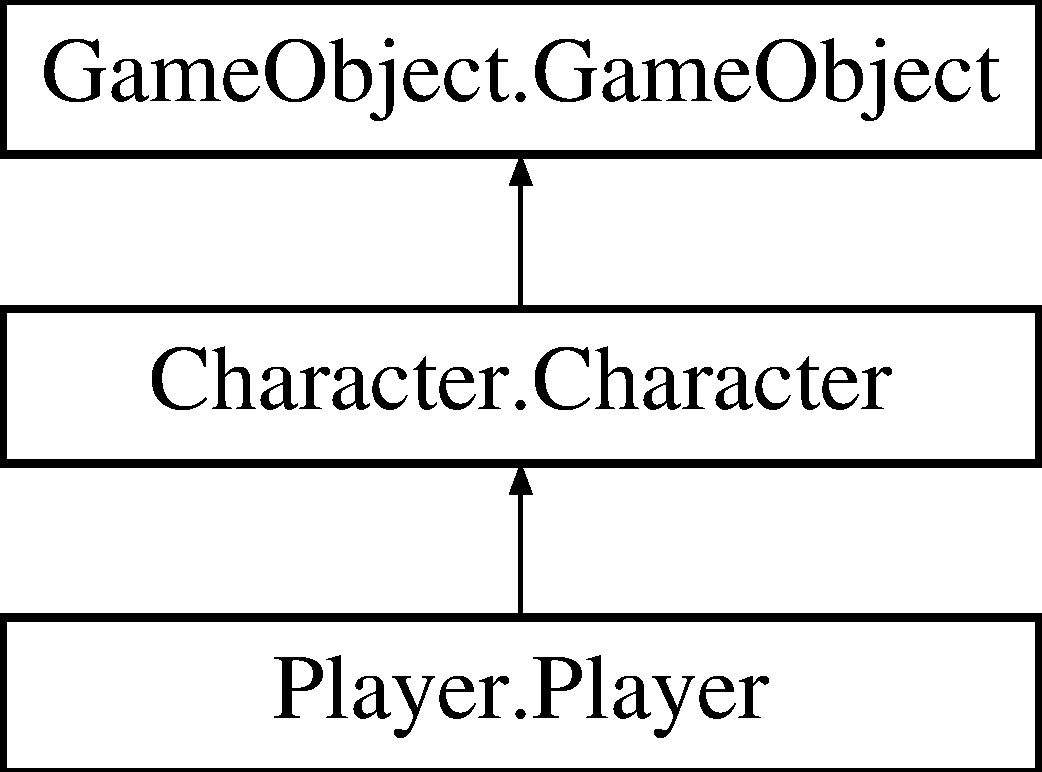
\includegraphics[height=3.000000cm]{classPlayer_1_1Player}
\end{center}
\end{figure}


\subsection{\-Detailed \-Description}
\begin{DoxyVerb}A Character that has its inputs from a real person. To be inherited by
a more specific class. At the time there are TVPlayers and HomePlayers
\end{DoxyVerb}
 

\-The documentation for this class was generated from the following file\-:\begin{DoxyCompactItemize}
\item 
\-Player.\-py\end{DoxyCompactItemize}

\hypertarget{classGame_1_1Poll}{\section{\-Game.\-Poll \-Class \-Reference}
\label{classGame_1_1Poll}\index{\-Game.\-Poll@{\-Game.\-Poll}}
}
\subsection*{\-Public \-Member \-Functions}
\begin{DoxyCompactItemize}
\item 
def \hyperlink{classGame_1_1Poll_afd96f4b0f4e4803b3da6f6494260d41c}{\-\_\-\-\_\-init\-\_\-\-\_\-}
\item 
def \hyperlink{classGame_1_1Poll_a3903be442b757965fe2a7ca00fc5aab7}{compute\-Vote}
\item 
def \hyperlink{classGame_1_1Poll_a4a6669f245973c3ef9565536ac055b97}{get\-Rank}
\item 
def \hyperlink{classGame_1_1Poll_a9667b4caa7ba397619c2bd2c4e7335e5}{get\-Winner}
\item 
def \hyperlink{classGame_1_1Poll_aff874d58fa1ee3c910abd1db950eebdd}{new\-Turn}
\item 
def \hyperlink{classGame_1_1Poll_a4d48a1823d18cba288b31ac2140cd0b3}{formattedstr}
\item 
def \hyperlink{classGame_1_1Poll_a932dcfa2b6ff73fb8f85b80ba146c004}{introduction}
\item 
def \hyperlink{classGame_1_1Poll_aabcf28c68c480a68fdd541907049481b}{catching\-Up}
\end{DoxyCompactItemize}
\subsection*{\-Public \-Attributes}
\begin{DoxyCompactItemize}
\item 
\hypertarget{classGame_1_1Poll_ab2a518ed49b8954328633a6688f92eba}{\hyperlink{classGame_1_1Poll_ab2a518ed49b8954328633a6688f92eba}{question}}\label{classGame_1_1Poll_ab2a518ed49b8954328633a6688f92eba}

\begin{DoxyCompactList}\small\item\em \-The question for which the \hyperlink{classGame_1_1Poll}{\-Poll} is computing votes. \end{DoxyCompactList}\item 
\hypertarget{classGame_1_1Poll_a0ee0be48aad1272d32183d5a7225d9d9}{\hyperlink{classGame_1_1Poll_a0ee0be48aad1272d32183d5a7225d9d9}{data}}\label{classGame_1_1Poll_a0ee0be48aad1272d32183d5a7225d9d9}

\begin{DoxyCompactList}\small\item\em \-The list of possible answers, each one with a possible object attached and the number of votes received. \end{DoxyCompactList}\item 
\hypertarget{classGame_1_1Poll_aab48c01def4aaceda096f10c54dc1af4}{\hyperlink{classGame_1_1Poll_aab48c01def4aaceda096f10c54dc1af4}{turns}}\label{classGame_1_1Poll_aab48c01def4aaceda096f10c54dc1af4}

\begin{DoxyCompactList}\small\item\em \-The number of turns left before the \hyperlink{classGame_1_1Poll}{\-Poll} expires. \end{DoxyCompactList}\item 
\hypertarget{classGame_1_1Poll_ae7e10eae049169a19fe46d49b32549ec}{\hyperlink{classGame_1_1Poll_ae7e10eae049169a19fe46d49b32549ec}{isactive}}\label{classGame_1_1Poll_ae7e10eae049169a19fe46d49b32549ec}

\begin{DoxyCompactList}\small\item\em \-Boolean to indicate if the \hyperlink{classGame_1_1Poll}{\-Poll} is active. \end{DoxyCompactList}\item 
\hypertarget{classGame_1_1Poll_abdbd477f2415fa8b1549eac2bfb4698c}{\hyperlink{classGame_1_1Poll_abdbd477f2415fa8b1549eac2bfb4698c}{fformat}}\label{classGame_1_1Poll_abdbd477f2415fa8b1549eac2bfb4698c}

\begin{DoxyCompactList}\small\item\em \-Function to format the strings to be displayed. \end{DoxyCompactList}\end{DoxyCompactItemize}


\subsection{\-Detailed \-Description}
\begin{DoxyVerb}A class that represents a poll.
It has a question, a list of possible answers
and the means to compute votes to these answers\end{DoxyVerb}
 

\subsection{\-Constructor \& \-Destructor \-Documentation}
\hypertarget{classGame_1_1Poll_afd96f4b0f4e4803b3da6f6494260d41c}{\index{\-Game\-::\-Poll@{\-Game\-::\-Poll}!\-\_\-\-\_\-init\-\_\-\-\_\-@{\-\_\-\-\_\-init\-\_\-\-\_\-}}
\index{\-\_\-\-\_\-init\-\_\-\-\_\-@{\-\_\-\-\_\-init\-\_\-\-\_\-}!Game::Poll@{\-Game\-::\-Poll}}
\subsubsection[{\-\_\-\-\_\-init\-\_\-\-\_\-}]{\setlength{\rightskip}{0pt plus 5cm}def {\bf \-Game.\-Poll.\-\_\-\-\_\-init\-\_\-\-\_\-} (
\begin{DoxyParamCaption}
\item[{}]{self, }
\item[{}]{question, }
\item[{}]{answersobjs, }
\item[{}]{turns = {\ttfamily \-I\-N\-D\-E\-F}, }
\item[{}]{isactive = {\ttfamily \-True}, }
\item[{}]{fformat = {\ttfamily lambda~x\-:~\-None}}
\end{DoxyParamCaption}
)}}\label{classGame_1_1Poll_afd96f4b0f4e4803b3da6f6494260d41c}
\begin{DoxyVerb}Poll.__init__(self, question, answersobjs, turns = INDEF, isactive = True,
 fformat = lambda x: None
)

Initialization function

question is the question to be asked to the participants of the poll

answersobjs is a list of tuples (answer, obj).
Each answer can have an attached reference to any object.

turns is the number of turns for which the poll will remain active.
-1 is indefinite

isActive indicates whether of not the Poll is active

fformat if a function to format the answers and has a single argument,
the poll object itself and returns a list of formatted strings
\end{DoxyVerb}
 

\subsection{\-Member \-Function \-Documentation}
\hypertarget{classGame_1_1Poll_aabcf28c68c480a68fdd541907049481b}{\index{\-Game\-::\-Poll@{\-Game\-::\-Poll}!catching\-Up@{catching\-Up}}
\index{catching\-Up@{catching\-Up}!Game::Poll@{\-Game\-::\-Poll}}
\subsubsection[{catching\-Up}]{\setlength{\rightskip}{0pt plus 5cm}def {\bf \-Game.\-Poll.\-catching\-Up} (
\begin{DoxyParamCaption}
\item[{}]{self}
\end{DoxyParamCaption}
)}}\label{classGame_1_1Poll_aabcf28c68c480a68fdd541907049481b}
\begin{DoxyVerb}Generates a JSON friendly dictionary with
all the object's attributes and values.
This function is intended as a update on the object's state,
sent to receivers that are already able to identify the object.
\end{DoxyVerb}
 \hypertarget{classGame_1_1Poll_a3903be442b757965fe2a7ca00fc5aab7}{\index{\-Game\-::\-Poll@{\-Game\-::\-Poll}!compute\-Vote@{compute\-Vote}}
\index{compute\-Vote@{compute\-Vote}!Game::Poll@{\-Game\-::\-Poll}}
\subsubsection[{compute\-Vote}]{\setlength{\rightskip}{0pt plus 5cm}def {\bf \-Game.\-Poll.\-compute\-Vote} (
\begin{DoxyParamCaption}
\item[{}]{self, }
\item[{}]{answer, }
\item[{}]{votes = {\ttfamily 1}}
\end{DoxyParamCaption}
)}}\label{classGame_1_1Poll_a3903be442b757965fe2a7ca00fc5aab7}
\begin{DoxyVerb}Poll.computeVote(self, answer, votes = 1)
Computes votes to one of the Polls answers
the answer can be either a string or the index in self.data
\end{DoxyVerb}
 \hypertarget{classGame_1_1Poll_a4d48a1823d18cba288b31ac2140cd0b3}{\index{\-Game\-::\-Poll@{\-Game\-::\-Poll}!formattedstr@{formattedstr}}
\index{formattedstr@{formattedstr}!Game::Poll@{\-Game\-::\-Poll}}
\subsubsection[{formattedstr}]{\setlength{\rightskip}{0pt plus 5cm}def {\bf \-Game.\-Poll.\-formattedstr} (
\begin{DoxyParamCaption}
\item[{}]{self}
\end{DoxyParamCaption}
)}}\label{classGame_1_1Poll_a4d48a1823d18cba288b31ac2140cd0b3}
\begin{DoxyVerb}Poll.formattedstr(self)
Returns a list of the Poll's formatted strings.
The first one being the question and the others the answers, in order
\end{DoxyVerb}
 \hypertarget{classGame_1_1Poll_a4a6669f245973c3ef9565536ac055b97}{\index{\-Game\-::\-Poll@{\-Game\-::\-Poll}!get\-Rank@{get\-Rank}}
\index{get\-Rank@{get\-Rank}!Game::Poll@{\-Game\-::\-Poll}}
\subsubsection[{get\-Rank}]{\setlength{\rightskip}{0pt plus 5cm}def {\bf \-Game.\-Poll.\-get\-Rank} (
\begin{DoxyParamCaption}
\item[{}]{self}
\end{DoxyParamCaption}
)}}\label{classGame_1_1Poll_a4a6669f245973c3ef9565536ac055b97}
\begin{DoxyVerb}Poll.getRank(self)
Returns the Poll's results ordered by most voted answers
\end{DoxyVerb}
 \hypertarget{classGame_1_1Poll_a9667b4caa7ba397619c2bd2c4e7335e5}{\index{\-Game\-::\-Poll@{\-Game\-::\-Poll}!get\-Winner@{get\-Winner}}
\index{get\-Winner@{get\-Winner}!Game::Poll@{\-Game\-::\-Poll}}
\subsubsection[{get\-Winner}]{\setlength{\rightskip}{0pt plus 5cm}def {\bf \-Game.\-Poll.\-get\-Winner} (
\begin{DoxyParamCaption}
\item[{}]{self}
\end{DoxyParamCaption}
)}}\label{classGame_1_1Poll_a9667b4caa7ba397619c2bd2c4e7335e5}
\begin{DoxyVerb}Poll.getWinner(self)
Returns the Poll's winning answer
\end{DoxyVerb}
 \hypertarget{classGame_1_1Poll_a932dcfa2b6ff73fb8f85b80ba146c004}{\index{\-Game\-::\-Poll@{\-Game\-::\-Poll}!introduction@{introduction}}
\index{introduction@{introduction}!Game::Poll@{\-Game\-::\-Poll}}
\subsubsection[{introduction}]{\setlength{\rightskip}{0pt plus 5cm}def {\bf \-Game.\-Poll.\-introduction} (
\begin{DoxyParamCaption}
\item[{}]{self}
\end{DoxyParamCaption}
)}}\label{classGame_1_1Poll_a932dcfa2b6ff73fb8f85b80ba146c004}
\begin{DoxyVerb}Generates a JSON friendly dictionary with
all the object's attributes and values.
This function is intended as a first introduction of the object,
to receivers that are unaware of its existence.
\end{DoxyVerb}
 \hypertarget{classGame_1_1Poll_aff874d58fa1ee3c910abd1db950eebdd}{\index{\-Game\-::\-Poll@{\-Game\-::\-Poll}!new\-Turn@{new\-Turn}}
\index{new\-Turn@{new\-Turn}!Game::Poll@{\-Game\-::\-Poll}}
\subsubsection[{new\-Turn}]{\setlength{\rightskip}{0pt plus 5cm}def {\bf \-Game.\-Poll.\-new\-Turn} (
\begin{DoxyParamCaption}
\item[{}]{self, }
\item[{}]{turnnumber = {\ttfamily 1}}
\end{DoxyParamCaption}
)}}\label{classGame_1_1Poll_aff874d58fa1ee3c910abd1db950eebdd}
\begin{DoxyVerb}Poll.newTurn(self, turnnumber = 1)
Function to compute a new turn
\end{DoxyVerb}
 

\-The documentation for this class was generated from the following file\-:\begin{DoxyCompactItemize}
\item 
\-Game.\-py\end{DoxyCompactItemize}

\hypertarget{classScript_1_1Script}{\section{\-Script.\-Script \-Class \-Reference}
\label{classScript_1_1Script}\index{\-Script.\-Script@{\-Script.\-Script}}
}
\subsection*{\-Public \-Member \-Functions}
\begin{DoxyCompactItemize}
\item 
\hypertarget{classScript_1_1Script_aaa7dd1905116549b57b5815417762ef1}{def {\bfseries \-\_\-\-\_\-init\-\_\-\-\_\-}}\label{classScript_1_1Script_aaa7dd1905116549b57b5815417762ef1}

\end{DoxyCompactItemize}
\subsection*{\-Public \-Attributes}
\begin{DoxyCompactItemize}
\item 
\hypertarget{classScript_1_1Script_a5953fa4e7305e0af72c5853a76c29698}{\hyperlink{classScript_1_1Script_a5953fa4e7305e0af72c5853a76c29698}{owner}}\label{classScript_1_1Script_a5953fa4e7305e0af72c5853a76c29698}

\begin{DoxyCompactList}\small\item\em \-The \hyperlink{namespaceGameObject}{\-Game\-Object} which the script affects. \end{DoxyCompactList}\item 
\hypertarget{classScript_1_1Script_a402bc01b65d4fbdcda8c04188df3b33e}{\hyperlink{classScript_1_1Script_a402bc01b65d4fbdcda8c04188df3b33e}{on\-Create}}\label{classScript_1_1Script_a402bc01b65d4fbdcda8c04188df3b33e}

\begin{DoxyCompactList}\small\item\em \-Function to be called once after the instantiation of self.\-owner. \end{DoxyCompactList}\item 
\hypertarget{classScript_1_1Script_a5011704e68cf5edaeb37f1640edacd65}{\hyperlink{classScript_1_1Script_a5011704e68cf5edaeb37f1640edacd65}{on\-Update}}\label{classScript_1_1Script_a5011704e68cf5edaeb37f1640edacd65}

\begin{DoxyCompactList}\small\item\em \-Function to be called at each turn. \end{DoxyCompactList}\item 
\hypertarget{classScript_1_1Script_aeb1b75f0e269eb9719dd775b96258d5b}{\hyperlink{classScript_1_1Script_aeb1b75f0e269eb9719dd775b96258d5b}{on\-Collision}}\label{classScript_1_1Script_aeb1b75f0e269eb9719dd775b96258d5b}

\begin{DoxyCompactList}\small\item\em \-Function to be called when self.\-owner collides with another \hyperlink{namespaceGameObject}{\-Game\-Object}. \end{DoxyCompactList}\item 
\hyperlink{classScript_1_1Script_a2005d9e06798af0c2c8e6fa2ca976fb6}{on\-Interaction}
\begin{DoxyCompactList}\small\item\em function to be called when self.\-owner suffers an interaction. \end{DoxyCompactList}\end{DoxyCompactItemize}


\subsection{\-Detailed \-Description}
\begin{DoxyVerb}Script to dictate behavior of a GameObject. onCreate, onUpdate, onCollision
and onInteraction functions are called by the game's main loop.
\end{DoxyVerb}
 

\subsection{\-Member \-Data \-Documentation}
\hypertarget{classScript_1_1Script_a2005d9e06798af0c2c8e6fa2ca976fb6}{\index{\-Script\-::\-Script@{\-Script\-::\-Script}!on\-Interaction@{on\-Interaction}}
\index{on\-Interaction@{on\-Interaction}!Script::Script@{\-Script\-::\-Script}}
\subsubsection[{on\-Interaction}]{\setlength{\rightskip}{0pt plus 5cm}{\bf \-Script.\-Script\-::on\-Interaction}}}\label{classScript_1_1Script_a2005d9e06798af0c2c8e6fa2ca976fb6}


function to be called when self.\-owner suffers an interaction. 

\-It must receive the object that started the \hyperlink{namespaceInteraction}{\-Interaction} as its argument 

\-The documentation for this class was generated from the following file\-:\begin{DoxyCompactItemize}
\item 
\-Script.\-py\end{DoxyCompactItemize}

\hypertarget{classTeam_1_1Team}{\section{\-Team.\-Team \-Class \-Reference}
\label{classTeam_1_1Team}\index{\-Team.\-Team@{\-Team.\-Team}}
}
\subsection*{\-Public \-Member \-Functions}
\begin{DoxyCompactItemize}
\item 
def \hyperlink{classTeam_1_1Team_a9a7d47b8c92036911b8de7def308c107}{update\-Score}
\item 
def \hyperlink{classTeam_1_1Team_a3e23b02741f89cf2a530522a340e21ab}{get\-Score}
\item 
def \hyperlink{classTeam_1_1Team_a6ff7995fb1950ca7246a09809982ea46}{\-\_\-\-\_\-init\-\_\-\-\_\-}
\item 
def \hyperlink{classTeam_1_1Team_a0b4fbdff85a79a9345d99958c5de87b0}{add\-Member}
\item 
def \hyperlink{classTeam_1_1Team_a1f9b5f26f806bed2ae6e35554719d4ff}{add\-Members}
\item 
def \hyperlink{classTeam_1_1Team_a37790104488b3c01a635635226cee5b6}{remove\-Member}
\item 
def \hyperlink{classTeam_1_1Team_a05a50256efe52eba988fbddf4a243e4f}{remove\-Members}
\item 
def \hyperlink{classTeam_1_1Team_a5bba620642e81d565a8af2bed2f30b9e}{member\-In}
\item 
def \hyperlink{classTeam_1_1Team_a276c4d4180f64c3cb08b8010880a9b9d}{introduction}
\item 
def \hyperlink{classTeam_1_1Team_aeebecaa4f6aa2e6f5b82ee47a9979261}{catching\-Up}
\end{DoxyCompactItemize}
\subsection*{\-Static \-Public \-Member \-Functions}
\begin{DoxyCompactItemize}
\item 
def \hyperlink{classTeam_1_1Team_a7e8c2ab43819f9811dc6c7a562fbc1a3}{get\-Team\-By\-Id}
\item 
def \hyperlink{classTeam_1_1Team_ad31e302fa77d88bf51a248bd01b2ae8c}{get\-Team\-By\-Name}
\end{DoxyCompactItemize}
\subsection*{\-Public \-Attributes}
\begin{DoxyCompactItemize}
\item 
\hypertarget{classTeam_1_1Team_a108717c9daf1d659227c27a94f1fc8a0}{\hyperlink{classTeam_1_1Team_a108717c9daf1d659227c27a94f1fc8a0}{score}}\label{classTeam_1_1Team_a108717c9daf1d659227c27a94f1fc8a0}

\begin{DoxyCompactList}\small\item\em \-The \hyperlink{classTeam_1_1Team}{\-Team}'s current score. \end{DoxyCompactList}\item 
\hypertarget{classTeam_1_1Team_a54bac45272111d4fd74fddf2c23bfa09}{\hyperlink{classTeam_1_1Team_a54bac45272111d4fd74fddf2c23bfa09}{teamid}}\label{classTeam_1_1Team_a54bac45272111d4fd74fddf2c23bfa09}

\begin{DoxyCompactList}\small\item\em \-The identification number of a \hyperlink{classTeam_1_1Team}{\-Team}. \end{DoxyCompactList}\item 
\hypertarget{classTeam_1_1Team_a229f25a8d4687825dbb5756f556c0780}{\hyperlink{classTeam_1_1Team_a229f25a8d4687825dbb5756f556c0780}{name}}\label{classTeam_1_1Team_a229f25a8d4687825dbb5756f556c0780}

\begin{DoxyCompactList}\small\item\em \-The \hyperlink{classTeam_1_1Team}{\-Team}'s name. \end{DoxyCompactList}\item 
\hypertarget{classTeam_1_1Team_a1f45f57ffe8ebf1bfde387167a6859b5}{\hyperlink{classTeam_1_1Team_a1f45f57ffe8ebf1bfde387167a6859b5}{members}}\label{classTeam_1_1Team_a1f45f57ffe8ebf1bfde387167a6859b5}

\begin{DoxyCompactList}\small\item\em \-A list of \-Game\-Objects that are members of the \hyperlink{classTeam_1_1Team}{\-Team}. \end{DoxyCompactList}\item 
\hyperlink{classTeam_1_1Team_a01dc47fa71d0ee9d33a5bbd704d94e5a}{fscore}
\begin{DoxyCompactList}\small\item\em \-A function to calculate the \hyperlink{classTeam_1_1Team}{\-Team}'s current score. \end{DoxyCompactList}\end{DoxyCompactItemize}
\subsection*{\-Static \-Public \-Attributes}
\begin{DoxyCompactItemize}
\item 
\hypertarget{classTeam_1_1Team_a2a381be35594f58355daa36609d5d327}{list \hyperlink{classTeam_1_1Team_a2a381be35594f58355daa36609d5d327}{teams} = \mbox{[}$\,$\mbox{]}}\label{classTeam_1_1Team_a2a381be35594f58355daa36609d5d327}

\begin{DoxyCompactList}\small\item\em \-Static list with all the teams. \end{DoxyCompactList}\end{DoxyCompactItemize}


\subsection{\-Detailed \-Description}
\begin{DoxyVerb}Represents a Team of GameObjects\end{DoxyVerb}
 

\subsection{\-Constructor \& \-Destructor \-Documentation}
\hypertarget{classTeam_1_1Team_a6ff7995fb1950ca7246a09809982ea46}{\index{\-Team\-::\-Team@{\-Team\-::\-Team}!\-\_\-\-\_\-init\-\_\-\-\_\-@{\-\_\-\-\_\-init\-\_\-\-\_\-}}
\index{\-\_\-\-\_\-init\-\_\-\-\_\-@{\-\_\-\-\_\-init\-\_\-\-\_\-}!Team::Team@{\-Team\-::\-Team}}
\subsubsection[{\-\_\-\-\_\-init\-\_\-\-\_\-}]{\setlength{\rightskip}{0pt plus 5cm}def {\bf \-Team.\-Team.\-\_\-\-\_\-init\-\_\-\-\_\-} (
\begin{DoxyParamCaption}
\item[{}]{self, }
\item[{}]{teamid, }
\item[{}]{name, }
\item[{}]{initialmembers, }
\item[{}]{fscore = {\ttfamily lambda~members\-:~sum(~\mbox{[}member.score~for~member~in~{\bf members}\mbox{]}~)}}
\end{DoxyParamCaption}
)}}\label{classTeam_1_1Team_a6ff7995fb1950ca7246a09809982ea46}
\begin{DoxyVerb}Team.__init__(self,
      teamid,
      name,
      initialmembers = [],
      fscore = lambda t: sum( [p.score for p in t.members] ),
      initialscore = 0
     )
Initialization function for a Team object

teamid is an identification number for the team
name is the team's name
initialmembers is a initial list of team members (Character objects)

fscore is a function to calculate the teams score. it MUST receive
a Team object as its only parameter and return the teams score.
It MUST NOT update the teams score internally.
\end{DoxyVerb}
 

\subsection{\-Member \-Function \-Documentation}
\hypertarget{classTeam_1_1Team_a0b4fbdff85a79a9345d99958c5de87b0}{\index{\-Team\-::\-Team@{\-Team\-::\-Team}!add\-Member@{add\-Member}}
\index{add\-Member@{add\-Member}!Team::Team@{\-Team\-::\-Team}}
\subsubsection[{add\-Member}]{\setlength{\rightskip}{0pt plus 5cm}def {\bf \-Team.\-Team.\-add\-Member} (
\begin{DoxyParamCaption}
\item[{}]{self, }
\item[{}]{member}
\end{DoxyParamCaption}
)}}\label{classTeam_1_1Team_a0b4fbdff85a79a9345d99958c5de87b0}
\begin{DoxyVerb}Team.addMember(self, member)
Function to add a team member (Character object) to a Team object
returns True if the member is inserted and False otherwise.
Raises an assertionerror if member is not an instance of GameObject
\end{DoxyVerb}
 \hypertarget{classTeam_1_1Team_a1f9b5f26f806bed2ae6e35554719d4ff}{\index{\-Team\-::\-Team@{\-Team\-::\-Team}!add\-Members@{add\-Members}}
\index{add\-Members@{add\-Members}!Team::Team@{\-Team\-::\-Team}}
\subsubsection[{add\-Members}]{\setlength{\rightskip}{0pt plus 5cm}def {\bf \-Team.\-Team.\-add\-Members} (
\begin{DoxyParamCaption}
\item[{}]{self, }
\item[{}]{members}
\end{DoxyParamCaption}
)}}\label{classTeam_1_1Team_a1f9b5f26f806bed2ae6e35554719d4ff}
\begin{DoxyVerb}Team.addMembers(self, members)
Adds a list of members (Character object) to a Team object
If the list contains objects already in the list,
those objects will not be added
\end{DoxyVerb}
 \hypertarget{classTeam_1_1Team_aeebecaa4f6aa2e6f5b82ee47a9979261}{\index{\-Team\-::\-Team@{\-Team\-::\-Team}!catching\-Up@{catching\-Up}}
\index{catching\-Up@{catching\-Up}!Team::Team@{\-Team\-::\-Team}}
\subsubsection[{catching\-Up}]{\setlength{\rightskip}{0pt plus 5cm}def {\bf \-Team.\-Team.\-catching\-Up} (
\begin{DoxyParamCaption}
\item[{}]{self}
\end{DoxyParamCaption}
)}}\label{classTeam_1_1Team_aeebecaa4f6aa2e6f5b82ee47a9979261}
\begin{DoxyVerb}Generates a JSON friendly dictionary with
all the object's attributes and values.
This function is intended as a update on the object's state,
sent to receivers that are already able to identify the object.
\end{DoxyVerb}
 \hypertarget{classTeam_1_1Team_a3e23b02741f89cf2a530522a340e21ab}{\index{\-Team\-::\-Team@{\-Team\-::\-Team}!get\-Score@{get\-Score}}
\index{get\-Score@{get\-Score}!Team::Team@{\-Team\-::\-Team}}
\subsubsection[{get\-Score}]{\setlength{\rightskip}{0pt plus 5cm}def {\bf \-Team.\-Team.\-get\-Score} (
\begin{DoxyParamCaption}
\item[{}]{self}
\end{DoxyParamCaption}
)}}\label{classTeam_1_1Team_a3e23b02741f89cf2a530522a340e21ab}
\begin{DoxyVerb}Team.getScore(self)
The Team's current score
\end{DoxyVerb}
 \hypertarget{classTeam_1_1Team_a7e8c2ab43819f9811dc6c7a562fbc1a3}{\index{\-Team\-::\-Team@{\-Team\-::\-Team}!get\-Team\-By\-Id@{get\-Team\-By\-Id}}
\index{get\-Team\-By\-Id@{get\-Team\-By\-Id}!Team::Team@{\-Team\-::\-Team}}
\subsubsection[{get\-Team\-By\-Id}]{\setlength{\rightskip}{0pt plus 5cm}def {\bf \-Team.\-Team.\-get\-Team\-By\-Id} (
\begin{DoxyParamCaption}
\item[{}]{teamid}
\end{DoxyParamCaption}
)\hspace{0.3cm}{\ttfamily  \mbox{[}static\mbox{]}}}}\label{classTeam_1_1Team_a7e8c2ab43819f9811dc6c7a562fbc1a3}
\begin{DoxyVerb}Team.getTeamById(teamid)
Returns the team in Team.teams whose teamid matches the argument
or None for no match.
\end{DoxyVerb}
 \hypertarget{classTeam_1_1Team_ad31e302fa77d88bf51a248bd01b2ae8c}{\index{\-Team\-::\-Team@{\-Team\-::\-Team}!get\-Team\-By\-Name@{get\-Team\-By\-Name}}
\index{get\-Team\-By\-Name@{get\-Team\-By\-Name}!Team::Team@{\-Team\-::\-Team}}
\subsubsection[{get\-Team\-By\-Name}]{\setlength{\rightskip}{0pt plus 5cm}def {\bf \-Team.\-Team.\-get\-Team\-By\-Name} (
\begin{DoxyParamCaption}
\item[{}]{name}
\end{DoxyParamCaption}
)\hspace{0.3cm}{\ttfamily  \mbox{[}static\mbox{]}}}}\label{classTeam_1_1Team_ad31e302fa77d88bf51a248bd01b2ae8c}
\begin{DoxyVerb}Team.getTeamByName(name)
Returns the team in Team.teams whose name matches the argument
or None for no match.
\end{DoxyVerb}
 \hypertarget{classTeam_1_1Team_a276c4d4180f64c3cb08b8010880a9b9d}{\index{\-Team\-::\-Team@{\-Team\-::\-Team}!introduction@{introduction}}
\index{introduction@{introduction}!Team::Team@{\-Team\-::\-Team}}
\subsubsection[{introduction}]{\setlength{\rightskip}{0pt plus 5cm}def {\bf \-Team.\-Team.\-introduction} (
\begin{DoxyParamCaption}
\item[{}]{self}
\end{DoxyParamCaption}
)}}\label{classTeam_1_1Team_a276c4d4180f64c3cb08b8010880a9b9d}
\begin{DoxyVerb}Generates a JSON friendly dictionary with
all the object's attributes and values.
This function is intended as a first introduction of the object,
to receivers that are unaware of its existence.
\end{DoxyVerb}
 \hypertarget{classTeam_1_1Team_a5bba620642e81d565a8af2bed2f30b9e}{\index{\-Team\-::\-Team@{\-Team\-::\-Team}!member\-In@{member\-In}}
\index{member\-In@{member\-In}!Team::Team@{\-Team\-::\-Team}}
\subsubsection[{member\-In}]{\setlength{\rightskip}{0pt plus 5cm}def {\bf \-Team.\-Team.\-member\-In} (
\begin{DoxyParamCaption}
\item[{}]{self, }
\item[{}]{member}
\end{DoxyParamCaption}
)}}\label{classTeam_1_1Team_a5bba620642e81d565a8af2bed2f30b9e}
\begin{DoxyVerb}Team.memberIn(self, member)
Returns True if member is in the Team and False otherwise.
Raises an assertionError if member is not a GameObject
\end{DoxyVerb}
 \hypertarget{classTeam_1_1Team_a37790104488b3c01a635635226cee5b6}{\index{\-Team\-::\-Team@{\-Team\-::\-Team}!remove\-Member@{remove\-Member}}
\index{remove\-Member@{remove\-Member}!Team::Team@{\-Team\-::\-Team}}
\subsubsection[{remove\-Member}]{\setlength{\rightskip}{0pt plus 5cm}def {\bf \-Team.\-Team.\-remove\-Member} (
\begin{DoxyParamCaption}
\item[{}]{self, }
\item[{}]{member}
\end{DoxyParamCaption}
)}}\label{classTeam_1_1Team_a37790104488b3c01a635635226cee5b6}
\begin{DoxyVerb}Team.removeMember(self, member)
Removes a member from a Team object.
Returns True for success and False for failure
\end{DoxyVerb}
 \hypertarget{classTeam_1_1Team_a05a50256efe52eba988fbddf4a243e4f}{\index{\-Team\-::\-Team@{\-Team\-::\-Team}!remove\-Members@{remove\-Members}}
\index{remove\-Members@{remove\-Members}!Team::Team@{\-Team\-::\-Team}}
\subsubsection[{remove\-Members}]{\setlength{\rightskip}{0pt plus 5cm}def {\bf \-Team.\-Team.\-remove\-Members} (
\begin{DoxyParamCaption}
\item[{}]{self, }
\item[{}]{members}
\end{DoxyParamCaption}
)}}\label{classTeam_1_1Team_a05a50256efe52eba988fbddf4a243e4f}
\begin{DoxyVerb}Team.removeMembers(self, members)
Removes a list of members (Character object) from a Team object.
If the list contains objects not in the list they are ignored
\end{DoxyVerb}
 \hypertarget{classTeam_1_1Team_a9a7d47b8c92036911b8de7def308c107}{\index{\-Team\-::\-Team@{\-Team\-::\-Team}!update\-Score@{update\-Score}}
\index{update\-Score@{update\-Score}!Team::Team@{\-Team\-::\-Team}}
\subsubsection[{update\-Score}]{\setlength{\rightskip}{0pt plus 5cm}def {\bf \-Team.\-Team.\-update\-Score} (
\begin{DoxyParamCaption}
\item[{}]{self}
\end{DoxyParamCaption}
)}}\label{classTeam_1_1Team_a9a7d47b8c92036911b8de7def308c107}
\begin{DoxyVerb}Team.updateScore(self)
Function that calculates the team's score
\end{DoxyVerb}
 

\subsection{\-Member \-Data \-Documentation}
\hypertarget{classTeam_1_1Team_a01dc47fa71d0ee9d33a5bbd704d94e5a}{\index{\-Team\-::\-Team@{\-Team\-::\-Team}!fscore@{fscore}}
\index{fscore@{fscore}!Team::Team@{\-Team\-::\-Team}}
\subsubsection[{fscore}]{\setlength{\rightskip}{0pt plus 5cm}{\bf \-Team.\-Team\-::fscore}}}\label{classTeam_1_1Team_a01dc47fa71d0ee9d33a5bbd704d94e5a}


\-A function to calculate the \hyperlink{classTeam_1_1Team}{\-Team}'s current score. 

\-It \-M\-U\-S\-T \-N\-O\-T set the value of self.\-score internally, but just return a value self.\-members must be its only argument 

\-The documentation for this class was generated from the following file\-:\begin{DoxyCompactItemize}
\item 
\-Team.\-py\end{DoxyCompactItemize}

\printindex
\end{document}
